\documentclass[journal]{IEEEtran}

\usepackage{amsmath,amssymb}
\usepackage{booktabs}
\usepackage{graphicx}
\usepackage{multirow}
\usepackage{url}
\usepackage{xcolor}
\usepackage{cite}
\usepackage{microtype}

\graphicspath{{figures/}}
\newcommand{\method}{DQA-ARC}
\newcommand{\etal}{et al.}
\newcommand{\artifacturl}{\url{https://github.com/Mi12Mi12Cu/DQA-ARC}}

\title{Deadline- and Quality-Aware Application-State Control for MQTT--LLM Pipelines}

\author{Miracle Udurume, Vladimir Shakhov, and Insoo Koo%
\thanks{M. Udurume and I. Koo are with the Department of Electrical, Electronics and Computer Engineering, University of Ulsan, Ulsan, Republic of Korea (e-mail: udurumemiracle@gmail.com; iskoo@ulsan.ac.kr).}%
\thanks{V. Shakhov is with the Institute for Information Transmission Problems (IITP RAS), Russian Academy of Sciences, Moscow, Russia (e-mail: Vladimir.Shakhov@gmail.com).}}

\begin{document}
\maketitle

\begin{abstract}
MQTT brokers acknowledge protocol delivery, not completion of downstream large-language-model (LLM) inference. A system that retains state until inference finishes therefore needs an explicit application-layer completion mechanism. We present the Deadline- and Quality-Aware Application-state Retention Controller (\method{}) for bounded application state in MQTT--LLM pipelines. MQTT~5 Response Topic and Correlation Data properties carry a separate completion message, while a co-located controller releases each admitted record on correlated completion or expiry. An Erlang--B calculation supplies a conditional feedforward budget; the controller maps that budget to a deadline by inverting the empirical truncated mean of measured completion time, adds blocking feedback, enforces class-specific latency floors, and may reroute work across GPU and CPU-only execution classes. Subscribers choose among measured prompt/output configurations by held-out task accuracy subject to a tail-latency constraint, and full context-window use is optional.

We implement the design with Mosquitto~2.1.2, MQTT~5/QoS~1 clients, and Ollama~0.40.14. Of 522 executed live broker--LLM runs, 430 belong to the prespecified analysis matrices; the study also contains 10,800 profiled inferences across Qwen2.5--1.5B/3B/7B and Llama~3.1--8B and 9,800 empirical-replay runs. Across ten paired seeds during simultaneous arrival-rate/model-service drift, \method{} gains 0.527 correct on-time results/s over prespecified occupancy-threshold admission, 0.267/s over FIFO operation without proactive admission, and 1.273/s over combined threshold/reservation control (all two-sided exact $p=0.00195$). Its advantage over the occupancy baseline remains 0.407/s across a four-value threshold sensitivity analysis (Holm-adjusted $p=0.00781$). The result is not universal dominance: under MMPP, the least restrictive tested occupancy threshold and FIFO yield 0.279/s and 0.302/s more goodput, respectively, by rejecting or expiring work at different stages. A fixed-deadline sweep likewise shows no guarded advantage over the best fixed value in stationary traffic. Class-conditioned allocation beats static compact selection but not maximum-context or token-max selection on the live Qwen2.5--3B study. The results locate the controller's benefit in changing-load conditions and quantify its blocking--expiry trade-off under bursts.
\end{abstract}

\begin{IEEEkeywords}
MQTT, large language models, admission control, deadline control, heterogeneous inference, empirical calibration.
\end{IEEEkeywords}

% BEGIN INLINED sections/01_introduction.tex
\section{Introduction}
\label{sec:introduction}

MQTT is a lightweight publish--subscribe protocol used across monitoring, industrial, transportation, home, and smart-city deployments. A recent Internet-wide measurement found 14,386 publicly reachable brokers and collected 3.2~billion messages, confirming both broad use and substantial diversity in topic and traffic behavior~\cite{innamorati2026pulse}. Edge and gateway applications increasingly need to combine numeric telemetry with operator-written alarm descriptions, heterogeneous vendor logs, maintenance histories, and natural-language explanations. An LLM is useful when these inputs cannot be reduced to one fixed parser or threshold table, while exact action labels remain valuable for reproducible safety evaluation. This combination creates an end-to-end control problem: protocol delivery may be fast, while the application invoked by a delivered request may queue for a heterogeneous CPU/GPU resource and run for orders of magnitude longer.

MQTT delivery and application completion have distinct semantics. In MQTT QoS~1, PUBACK transfers protocol responsibility for an Application Message. It does not report that the receiving subscriber has completed the action encoded by that message; indeed, MQTT does not require onward delivery to finish before PUBACK is sent~\cite{oasis2019mqtt}. MQTT~5 supplies a request/response pattern through Response Topic and Correlation Data, but the broker treats the request and response as ordinary Application Messages. Message Expiry Interval prevents stale undelivered messages from being forwarded indefinitely; it does not retain a delivered request until LLM execution finishes. Consequently, completion-aware retention requires application state separate from standard acknowledgment state.

We address this problem with the \emph{Deadline- and Quality-Aware Application-state Retention Controller} (\method{}), a distinct bounded controller co-located with the broker. A publisher sends a normal MQTT~5 request. The controller admits a record if capacity remains, forwards the job with an application deadline, and releases the record on the first correlated completion or expiry. This record store is the controlled resource. Rejection at this store is termed \emph{application-state blocking} and is distinct from MQTT packet loss and native in-flight blocking.

The second difficulty is model mismatch. Erlang--B gives an interpretable loss budget under locally stationary Poisson arrivals and independent holding times, but an exact inversion of that formula cannot itself demonstrate that a deployed system meets a target. IoT aggregates can be approximately Poisson only under scale, independence, and synchronization conditions~\cite{metzger2019modeling,lopez2020aggregated}; alarm storms and event-triggered sources can be bursty. LLM completion time is also configuration-, hardware-, queue-, and output-dependent. \method{} uses Erlang--B as a feedforward component, converts its mean holding-time budget into a deadline using measured completion samples, and corrects the deadline with observed blocking. A guard adds class-specific minimum budgets and load-aware routing when the common loss-model deadline would make useful completion infeasible.

Finally, longer prompts and outputs are not synonymous with higher task utility. Long-context studies report performance degradation with distractors and position effects~\cite{liu2024lost,hsieh2024ruler}, while LLM-serving systems explicitly separate prefill and decode costs and optimize latency/goodput rather than token count alone~\cite{kwon2023vllm,agrawal2024sarathi,zhong2024distserve}. Our subscriber therefore selects a measured configuration by held-out strict task accuracy subject to its tail-latency budget. The context limit is an inequality; unused context and early completion are valid outcomes.

The contributions are as follows.

\begin{itemize}
  \item We define and implement a protocol-correct MQTT~5 request/completion path that separates PUBACK, Message Expiry, and correlated application completion, and controls a bounded application record store.
  \item We develop a measured controller that combines conditional Erlang--B feedforward, empirical truncated-mean inversion, blocking feedback, class-specific feasibility floors, and load-aware rerouting across heterogeneous execution classes.
  \item We formulate inference configuration as a finite class-conditioned selection problem using calibration correctness and profiled latency. The 240-item corpus includes direct readings, temporal histories, and heterogeneous logs, so different requests can require different context.
  \item We evaluate the complete loop using a real Mosquitto broker, three Qwen2.5 sizes, and a Llama-3.1--8B-class comparator. Ten paired replications per condition compare \method{} with occupancy-threshold admission, static class reservation, their combination, and FIFO operation without proactive admission under Poisson, MMPP, and simultaneous arrival-rate/model-service drift. Matched studies cover four allocation rules, a five-point fixed-deadline sweep, and a four-point occupancy-threshold sensitivity analysis.
  \item We characterize the operating region under model mismatch and burstiness. Empirical replay includes a bounded-delay token-bucket variant and reports shaper loss separately from broker blocking, while an explicit local stability condition states when the blocking-feedback subsystem converges.
\end{itemize}

The remainder of the paper reviews related work, defines the protocol and controlled state, presents the controller and subscriber policy, evaluates the implementation, and discusses limitations and deployment implications.
% END INLINED sections/01_introduction.tex
% BEGIN INLINED sections/02_related_work.tex
\section{Related Work}
\label{sec:related}

\subsection{MQTT Semantics and Broker Evaluation}

The MQTT~5 standard defines delivery control packets, Message Expiry Interval, Receive Maximum, and a non-normative request/response pattern based on Response Topic and Correlation Data~\cite{oasis2019mqtt}. Eclipse Mosquitto implements MQTT~5, 3.1.1, and 3.1 and exposes the relevant properties to clients~\cite{mosquitto2026manual}. These mechanisms carry the request, deadline metadata, and completion. The controller preserves MQTT QoS behavior and manages bounded application state above the protocol layer.

Existing MQTT studies examine traffic, security, and scalability from complementary perspectives. Innamorati \etal{} characterize billions of messages from public brokers~\cite{innamorati2026pulse}; Buccafurri \etal{} add end-to-end flow integrity while preserving publish--subscribe decoupling~\cite{buccafurri2024mqtt}; and recent distributed-broker experiments measure latency, overhead, and locality~\cite{rostamivand2025distributed}. MQTTLoader provides a reproducible methodology for measuring MQTT~5 broker throughput and latency across QoS and subscription settings~\cite{banno2021mqttloader}. These works motivate realistic broker measurements but do not bind a delivered message to completion of an external inference job. Our focus is narrower: protocol-correct correlated completion plus control of the finite application records associated with outstanding AI work.

\subsection{IoT Arrival Models and Loss Systems}

The Palm--Khintchine argument is often invoked for aggregates of many independent, individually small sources, yet IoT source behavior is application dependent. Metzger \etal{} derive conditions and approximation errors for aggregated periodic IoT traffic~\cite{metzger2019modeling}; L\'opez-Ben\'itez \etal{} show that Poisson models can be inaccurate for finite collections of real sensor sources~\cite{lopez2020aggregated}; and Majumdar \etal{} experimentally test Poissonness for sensor data~\cite{majumdar2019poissonness}. These findings support using Poisson input as a conditional local model, not a universal description.

Loss networks provide the classical analytical basis for finite-capacity admission systems~\cite{kelly1991loss}. Erlang--B is insensitive to the holding-time distribution beyond its mean under its assumptions, but that result applies to the mathematical loss system, not automatically to a bursty, measured deployment. The MMPP captures rate modulation and correlated interarrivals while remaining analytically tractable~\cite{fischer1993mmpp}. We use Erlang--B to propose a mean holding-time budget and evaluate model violations separately with an MMPP, synchronized batches, and a rate step. Empirical calibration connects the abstract budget to actual completion samples.

\subsection{LLM Serving, Heterogeneity, and Context Quality}

Online inference systems established several principles used in our configuration and admission design. Clipper combines low-latency serving with adaptive model selection~\cite{crankshaw2017clipper}; Clockwork admits requests against latency SLOs using profiled execution behavior~\cite{gujarati2020clockwork}; and INFaaS selects among model and hardware variants using latency and accuracy requirements~\cite{romero2021infaas}. Standard token-bucket meters characterize admissible average rate and burst size~\cite{heinanen1999srtcm}; our burst-robust replay uses the same principle while exposing shaping delay and shaper drops separately.

Generative serving adds autoregressive execution, variable output length, and dynamic key/value state. Orca introduced iteration-level scheduling for generative Transformers~\cite{yu2022orca}, while vLLM uses PagedAttention to manage dynamic key/value memory~\cite{kwon2023vllm}. Sarathi-Serve uses chunked prefills to improve the throughput--latency trade-off~\cite{agrawal2024sarathi}; Splitwise and DistServe place prefill and decode on separately provisioned resources~\cite{patel2024splitwise,zhong2024distserve}; and Llumnix reschedules heterogeneous and unpredictable requests across instances~\cite{sun2024llumnix}. Mooncake extends disaggregation to long-context KV-cache storage under latency SLOs~\cite{qin2025mooncake}. More recent systems optimize resource overlap~\cite{zhu2025nanoflow}, unpredictable inference workloads~\cite{khare2025superserve}, and edge latency/energy trade-offs~\cite{tian2025clone}. EC-LLM similarly demonstrates that quality, latency, and cost must be evaluated together when routing between edge and cloud models~\cite{han2026ecllm}.

Our setting differs from datacenter schedulers in scale and control point: a lightweight MQTT gateway controls a small record store and dispatches to one GPU and one CPU-only execution class. We reuse the systems insight that heterogeneous requests require runtime measurement, while keeping the policy implementable as a profile lookup plus queue-aware routing.

Long-context quality is also nonmonotone. Liu \etal{} show that relevant information placed in the middle of a long context can be used less reliably~\cite{liu2024lost}, while RULER shows a gap between claimed and effective context length across many models~\cite{hsieh2024ruler}. These studies do not imply that short prompts are always better, but they invalidate an unconditional objective that fills the context window. Our controlled task includes archived, conflicting observations as distractors in the extended prompt and measures the effect on held-out decisions across Qwen2.5 and Llama~3.1~\cite{grattafiori2024llama3}.

\subsection{Positioning}

This work integrates four elements at the MQTT gateway: (i) a standards-compliant completion path, (ii) bounded application state, (iii) empirical conversion from a loss budget to an actionable deadline, and (iv) utility-aware inference selection with heterogeneous routing. This scope complements broker studies and general-purpose LLM serving systems by focusing on outstanding AI requests associated with delivered MQTT messages. Correctness, expiry, correlated completion, blocking under burstiness, and MQTT acknowledgment latency are measured independently of the analytical target.
% END INLINED sections/02_related_work.tex
% BEGIN INLINED sections/03_system_model.tex
\section{System and Protocol Model}
\label{sec:system}

\subsection{Entities and Controlled Resource}

The system contains publishers, an MQTT~5 broker, a co-located application-state controller, and LLM subscribers. The controller runs as a separate Node.js process on the broker host and manages \emph{gateway/application-state capacity}; Mosquitto's native in-flight store remains unchanged. Co-location removes an avoidable wide-area hop but is not required by the protocol.

For request $i$, the controller stores
\begin{equation}
 r_i=(id_i,c_i,t_i,D_i,x_i,z_i),
\end{equation}
where $id_i$ is the correlation identifier, $c_i\in\{g,c\}$ is the assigned GPU or CPU-only class, $t_i$ is admission time, $D_i$ is the application deadline, $x_i$ is the inference configuration, and $z_i$ is state. All records occupy one unit in this implementation; unequal byte sizes and multirate loss control are left to future work. With capacity $n$, an arrival that sees $n$ records is rejected immediately and receives an application response with status \texttt{blocked}.

Let $S_{i}$ be elapsed time from admission until the controller observes the correlated completion. It includes broker-to-subscriber delivery, subscriber queueing, inference, and result publication. The record holding time is
\begin{equation}
 H_i=\min(S_i,D_i).
 \label{eq:holding}
\end{equation}
If $S_i>D_i$, the record is released on expiry; a later result is logged as late and does not recreate state. Correct, on-time goodput counts completions that arrive before expiry, parse as valid JSON, and contain the correct task label.

\subsection{Protocol Sequence}

Figure~\ref{fig:sequence} shows the complete path. A publisher first subscribes to its response topic and sends a QoS~1 PUBLISH request containing Response Topic and Correlation Data. Mosquitto returns PUBACK according to MQTT rules. The controller independently receives the request event and either rejects it or creates $r_i$. On admission, it publishes a job to the selected subscriber-class topic with three MQTT~5 properties: Correlation Data, Message Expiry Interval, and User Properties encoding the application deadline, configuration, and class.

The subscriber processes the job and publishes the result with the same Correlation Data. The controller correlates the result, releases $r_i$, and publishes a completion response. If the timer fires first, it releases $r_i$ and publishes an expiry response. The publisher-facing response is therefore an application message, never PUBACK/PUBREC/PUBCOMP.

\begin{figure*}[t]
  \centering
  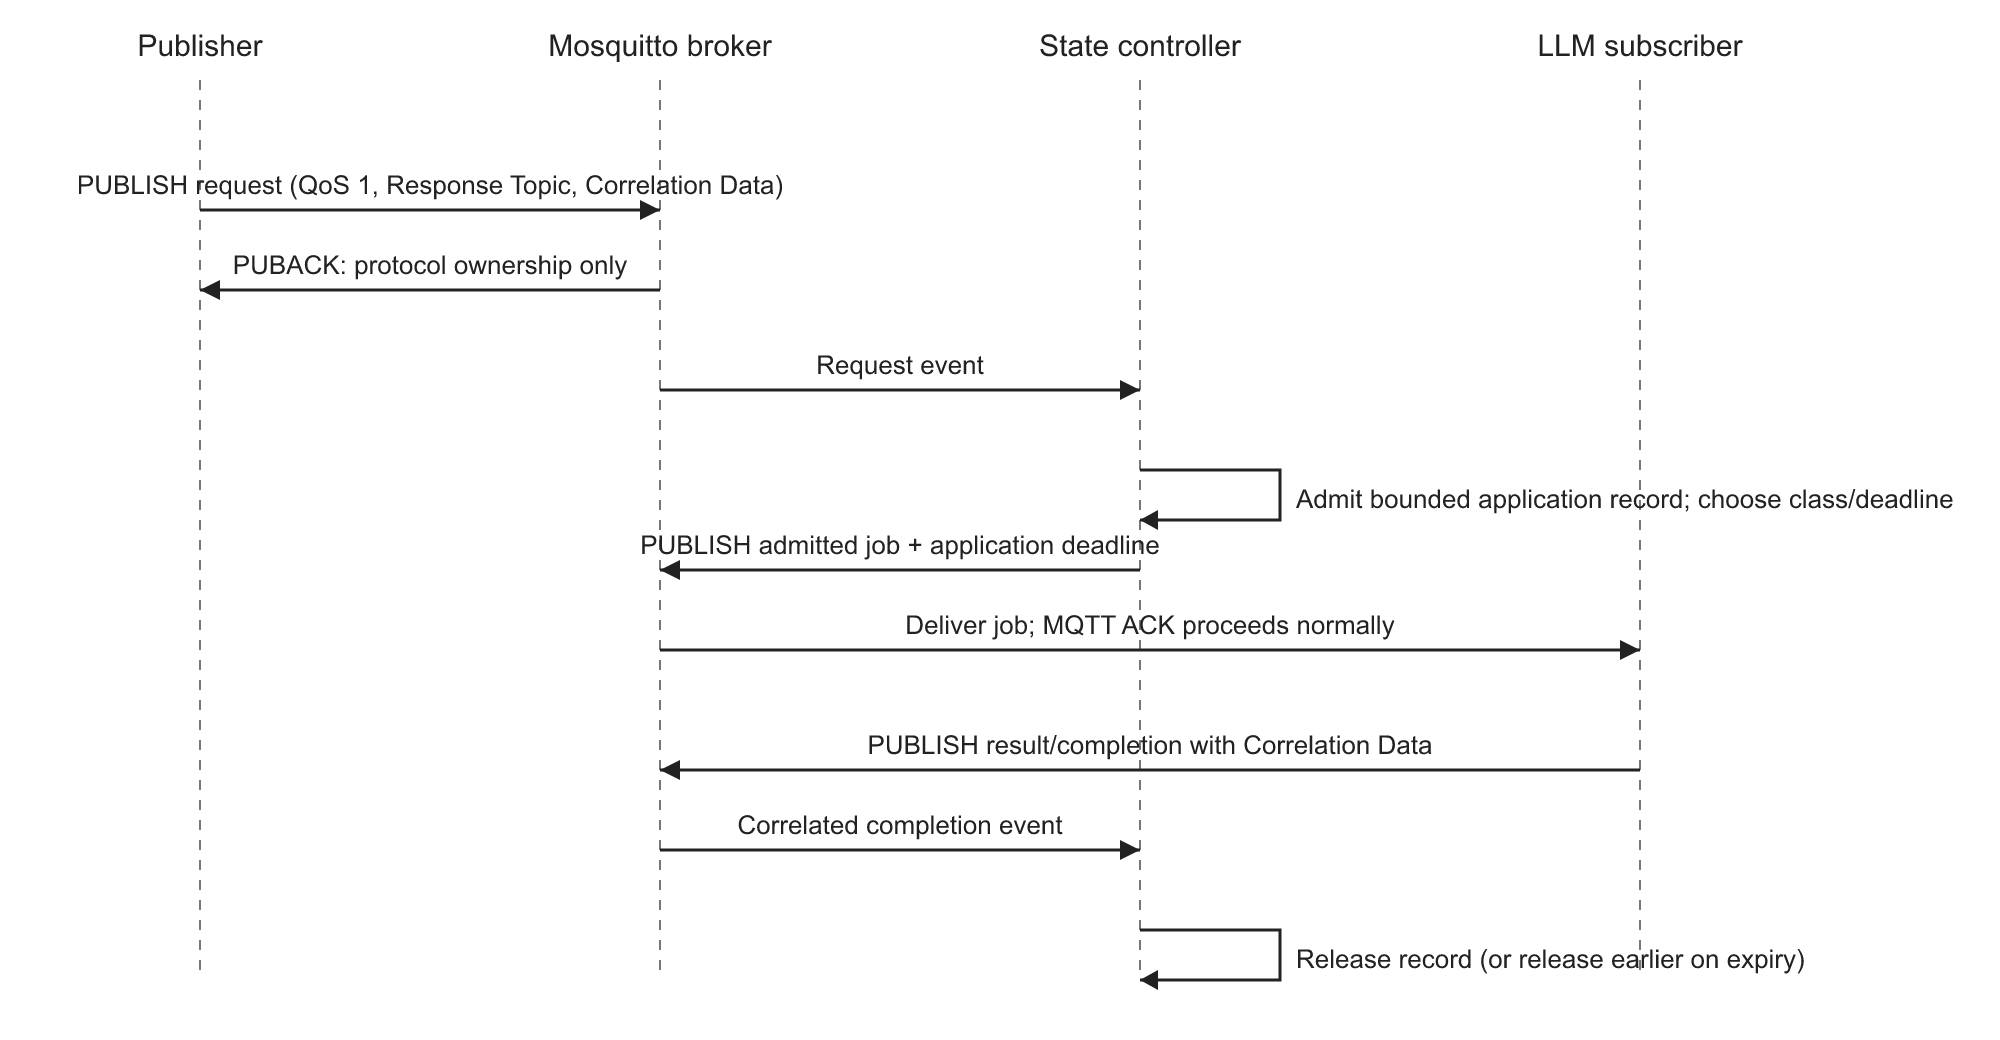
\includegraphics[width=0.98\textwidth]{fig5_mqtt_sequence.png}
  \caption{MQTT--LLM application-state control workflow. The MQTT QoS acknowledgment is independent of application-level completion. The controller maintains bounded request state and releases it upon correlated LLM completion or deadline expiry.}
  \label{fig:sequence}
\end{figure*}

Message Expiry Interval remains useful but has a narrower role. Per MQTT~5, the broker removes an expired message if onward delivery has not begun~\cite{oasis2019mqtt}. It does not keep a delivered request resident while an LLM executes. Equation~\eqref{eq:holding} is implemented by the controller's timer and completion correlation.

\subsection{Traffic and Subscriber Classes}

During a short control epoch $\Delta$, the feedforward model treats admitted attempts as a locally stationary Poisson process with rate $\lambda$. This approximation is intended for many independent, low-rate sources with randomized phases and no dominant source. Synchronized publishers, alarms, retries, and small source populations fall outside this regime. The implementation records the one-second index of dispersion
\begin{equation}
 I=\frac{\operatorname{Var}[N(1\ \mathrm{s})]}{\mathbb{E}[N(1\ \mathrm{s})]},
\end{equation}
and the evaluation treats large deviations from $I=1$ as evidence of mismatch rather than discarding the run.

The two subscriber classes execute the same model and task but use different Ollama endpoints: one may use the RTX~3060 GPU, while the other is explicitly forced to CPU-only execution on the same host. The principal live matrix uses Qwen2.5--3B, and the drift condition changes both endpoints to Qwen2.5--7B halfway through a run. This design isolates execution-class heterogeneity without falsely claiming two physical edge devices. Class preference is drawn independently for each arrival with CPU fraction $p_c$; the guarded policy may reroute a request if its preferred queue is predicted to miss a class-specific feasibility floor.

\subsection{Objective and Metrics}

The controller operates under three competing outcomes:
\begin{align}
 B_{\mathrm{app}} &= \frac{N_{\mathrm{blocked}}}{N_{\mathrm{published}}},\\
 E_{\mathrm{adm}} &= \frac{N_{\mathrm{expired}}}{N_{\mathrm{admitted}}},\\
 G_Q &= \frac{N_{\mathrm{correct,on\mbox{-}time}}}{T_{\mathrm{run}}}.
\end{align}
Reducing $D$ may reduce $B_{\mathrm{app}}$ while increasing $E_{\mathrm{adm}}$; increasing it may do the reverse. Hence blocking alone is not a sufficient objective. We report all three metrics, strict on-time accuracy, MQTT PUBACK latency, end-to-end completion latency, occupancy, rerouting, and process memory. The design goal is high $G_Q$ with explicit visibility into whether capacity is protected by successful completion, expiry, or admission shedding.
% END INLINED sections/03_system_model.tex
% BEGIN INLINED sections/04_controller.tex
\section{Deadline, Routing, and Quality Control}
\label{sec:controller}

\subsection{Conditional Loss-Model Feedforward}

For $n$ equal application records and offered load $A$, Erlang--B is evaluated by the stable recursion
\begin{equation}
 B_0(A)=1,\qquad B_j(A)=\frac{A B_{j-1}(A)}{j+A B_{j-1}(A)}.
 \label{eq:erlang-recursion}
\end{equation}
Numerical bisection gives $A_\alpha(n)$ such that $B_n(A_\alpha)=\alpha$. This computation is performed once per capacity/target pair; it is a model input, not an experimental result.

At epoch $k$, containing $N_k$ arrivals, the implementation updates
\begin{align}
 \widehat\lambda_k&=(1-\beta)\widehat\lambda_{k-1}+\beta N_k/\Delta,\\
 \lambda_k^{U}&=\widehat\lambda_k+z\sqrt{\max(\widehat\lambda_k,0.01)/\Delta},
 \label{eq:rate-upper}
\end{align}
with $\beta=0.5$ and $z=1.645$. Equation~\eqref{eq:rate-upper} is a one-sided Poisson-inspired margin, not a distribution-free confidence bound; its failure under MMPP traffic is measured in Section~\ref{sec:evaluation}. The feedforward mean holding-time budget is
\begin{equation}
 m_k^{\max}=\frac{A_\alpha(n)}{\lambda_k^{U}}.
 \label{eq:mean-budget}
\end{equation}

The \emph{analytical} baseline clips $D=m_k^{\max}$ directly. This equality is accurate only in a timeout-dominated regime; when jobs frequently finish before $D$, $\mathbb{E}[\min(S,D)]\neq D$. Comparing this baseline with empirical inversion quantifies the calibration error.

\subsection{Empirical Truncated-Mean Calibration}

For class $h$ and candidate configuration $x$, let $S_{h,x}$ denote measured completion time. From rolling samples $s_{h,x,1},\ldots,s_{h,x,M}$,
\begin{equation}
 \widehat m_{h,x}(D)=\frac{1}{M}\sum_{j=1}^{M}\min(s_{h,x,j},D).
 \label{eq:empirical-truncated}
\end{equation}
This estimator follows from
\begin{equation}
 \mathbb{E}[\min(S,D)]=\int_0^D \Pr(S>t)\,dt
\end{equation}
and is monotone in $D$. For current class fractions $p_{h,k}$ and selected configurations $x_h$, the calibrated feedforward deadline is the largest value in $[D_{\min},D_{\max}]$ satisfying
\begin{equation}
 \sum_h p_{h,k}\widehat m_{h,x_h}(D_k^{\mathrm{ff}})\le m_k^{\max}.
 \label{eq:mixture-inversion}
\end{equation}
The implementation solves~\eqref{eq:mixture-inversion} by bisection. Calibration profiles seed the estimator; completed live jobs are appended to a rolling window of 200 samples per class/configuration.

\subsection{Feedback and Rate Limiting}

Let $\widehat B_k$ be the epoch blocking fraction and
\begin{equation}
 \widetilde B_k=0.7\widetilde B_{k-1}+0.3\widehat B_k.
\end{equation}
The feedback candidate is
\begin{equation}
 D_{k+1}^{\mathrm{fb}}=\operatorname{clip}\left[
 D_k\exp\{\eta(\alpha-\widetilde B_k)\},D_{\min},D_{\max}\right]
 \label{eq:feedback}
\end{equation}
with $\eta=1.5$. The adaptive and guarded policies choose the more conservative of $D^{\mathrm{ff}}$ and $D^{\mathrm{fb}}$, then constrain one-epoch change to $[0.7D_k,1.3D_k]$. Every experiment uses $\Delta=4$~s, $D_{\min}=0.25$~s, and $D_{\max}=8$~s.

The following proposition states a local guarantee for the feedback component. It is deliberately conditional: no mean-rate controller can guarantee a target under arbitrary nonstationary bursts and finite capacity.

\textbf{Proposition 1 (local feedback stability).} Let $x_k=\log D_k$, let $b(x)$ be the differentiable steady blocking response near an unclipped equilibrium $x^*$ with $b(x^*)=\alpha$, and let $g=b'(x^*)>0$. If the feedforward minimum, clipping, and rate limiter are locally inactive, the smoothed feedback loop is locally asymptotically stable when
\begin{equation}
 0<\eta(1-a)g<2(1+a), \qquad a=0.7.
 \label{eq:stability-condition}
\end{equation}

\emph{Proof.} Linearizing the update that first forms $\widetilde B_{k+1}=a\widetilde B_k+(1-a)b(x_k)$ and then applies $x_{k+1}=x_k+\eta(\alpha-\widetilde B_{k+1})$ gives
\begin{equation}
 \begin{bmatrix}\delta x_{k+1}\\ \delta\widetilde B_{k+1}\end{bmatrix}
 =
 \begin{bmatrix}
 1-\eta(1-a)g & -\eta a\\
 (1-a)g & a
 \end{bmatrix}
 \begin{bmatrix}\delta x_k\\ \delta\widetilde B_k\end{bmatrix}.
\end{equation}
The matrix has determinant $a$ and trace $1+a-\eta(1-a)g$. The second-order Jury conditions yield $0<a<1$ and~\eqref{eq:stability-condition}. \hfill$\square$

Independently of this local condition, clipping makes $D_k\in[D_{\min},D_{\max}]$ invariant and the rate limiter bounds each multiplicative update. Section~\ref{sec:evaluation} estimates $g$ from the fixed-deadline sweep and evaluates the implemented gain. The \emph{adaptive} policy without a feasibility guard remains an ablation for measuring how a stable blocking loop can nevertheless choose deadlines below useful completion times.

\subsection{Class-Aware Feasibility Guard and Routing}

Mean-holding-time control can select a common deadline below the useful tail of a slow class. For a new request with $q_h$ jobs ahead of it, including an in-service job, the guarded policy uses the measured FIFO completion bound
\begin{equation}
 F_h(x,q_h)=\max\{D_{\min},Q_{0.95}(S_{h,x})+q_h\overline S_{h,x}+\delta_{\mathrm{msg}}\}.
 \label{eq:floors}
\end{equation}
Every term has a direct interpretation: one tail service time for the arriving job, mean measured service for work ahead, and a messaging/event-loop reserve. The implementation uses $\delta_{\mathrm{msg}}=0.05$~s; live event traces separately report the empirical p99 of end-to-end time minus subscriber wall time so this reserve can be audited.

The controller keeps the preferred class when $F_h\le D_{\max}$. Otherwise it selects a feasible alternative with the smallest normalized predicted workload; if neither class is feasible, it selects the smaller predicted completion time and records the infeasible admission. The admitted record receives
\begin{equation}
 D_i=\min\{D_{\max},\max(D_k,F_h(x_i,q_h))\}.
 \label{eq:record-deadline}
\end{equation}
Thus the common control state can respond to load, while a single slow class is not automatically assigned a deadline known to be infeasible. Admission capacity remains global; a route change does not create an additional record.

\subsection{Quality-Aware Inference Configuration}

The evaluated configuration set is
\begin{equation}
\begin{split}
 \mathcal X={}&\{\text{compact, standard, extended}\}\\
 &\times\{16,24,48\text{ output tokens}\}.
\end{split}
\end{equation}
Outputs below 16 tokens serve only as truncation checks and are not candidate configurations. Compact context contains the current numeric event; standard context adds the conditional history/log rules; extended context adds request-specific history or unstructured evidence together with archived distractors. For a configuration $x$, execution class $h$, task class $c$, and deadline $D_i$, feasibility requires
\begin{equation}
 \widehat Q_{0.95}(S_{h,x})+\delta\le D_i,\qquad \delta=0.05\ \mathrm{s}.
\end{equation}
Among feasible configurations, the subscriber selects the one with greatest calibration strict accuracy for task class $c$, then JSON validity, then smaller p95 latency and prompt size. Strict accuracy requires both the correct action and syntactically valid JSON. If none is feasible, the least-late candidate is used and the outcome remains visible in expiry/error metrics.

Three baselines characterize the effect of selection. \emph{Static compact} always selects compact--24, \emph{static maximum context} always selects extended--48, and \emph{token-max} selects the feasible candidate with the largest prompt-plus-output budget. None receives access to held-out labels. The live ablation compares all four allocators under identical traffic seeds and controller settings.

\subsection{Policy and Conventional Baseline Summary}

Three conventional admission rules provide comparators that do not use service profiles, feedback, or queue-aware rerouting. Let $o$ be current application-record occupancy, let $n=8$, let the fixed occupancy threshold be $\theta=\lceil0.75n\rceil=6$, and let $r=\lceil0.2n\rceil=2$ slots be reserved against the majority GPU-preferred class. CPU-preferred requests are the protected class because their measured service is slower and they comprise 20\% of arrivals. Both parameters were fixed before the test seeds: $\theta$ uses the common 75\%-occupancy headroom rule and $r$ matches the prespecified minority fraction; neither was selected from test outcomes. A separate sensitivity analysis evaluates $\theta\in\{4,5,6,7\}$ without replacing the prespecified $\theta=6$ headline baseline.

The \emph{occupancy-threshold} baseline (B1) admits either class iff $o<\theta$. The \emph{static-reservation} baseline (B2), a guard-channel rule from classical finite-capacity admission control~\cite{kelly1991loss}, admits CPU-preferred work iff $o<n$ and GPU-preferred work iff $o<n-r$. The \emph{threshold--reservation} baseline (B3) combines both restrictions: it admits CPU-preferred work iff $o<\theta$ and GPU-preferred work iff $o<\theta-r$. The FIFO reference has no proactive threshold or reservation: it admits in arrival order iff $o<n$ and rejects only at the hard record capacity. All four use the same profiled quality-aware inference allocator and fixed 8-s application deadline. Hence their comparison isolates admission/deadline control rather than prompt selection. ``No proactive admission'' does not mean unbounded state; the common eight-record safety bound remains enforced.

Table~\ref{tab:policies} separates the components.

\begin{table}[t]
\centering
\caption{Evaluated Deadline Policies}
\label{tab:policies}
\footnotesize
\begin{tabular}{@{}lccc@{}}
\toprule
Policy & Calibrated & Feedback & Class guard \\
\midrule
Fixed & no & no & no \\
Analytical & no ($D=m^{\max}$) & no & no \\
Calibrated & yes & no & no \\
Adaptive & yes & yes & no \\
Guarded (\method{}) & yes & yes & yes \\
\bottomrule
\end{tabular}
\end{table}

The deadline policies, conventional baselines, threshold-sensitivity cells, and FIFO reference share capacity, profile samples, and the same task/arrival trace in each paired seed. Their differences therefore reflect admission and deadline control rather than different offered workloads.
% END INLINED sections/04_controller.tex
% BEGIN INLINED sections/05_evaluation.tex
\section{Evaluation}
\label{sec:evaluation}

The evaluation asks seven questions. (Q1) How does class-conditioned configuration selection compare with compact, maximum-context, and token-max rules across models? (Q2) How do the five deadline policies behave under Poisson and bursty traffic? (Q3) Can a guarded controller improve upon the best fixed deadline when service time changes? (Q4) Does the implemented feedback gain satisfy the local stability condition? (Q5) What does protocol acknowledgment reveal about application completion? (Q6) Can bounded-delay token-bucket shaping make burst admission robust without merely relocating loss? (Q7) How does \method{} compare with occupancy-threshold admission, static class reservation, their combination, and FIFO operation without proactive admission, and are the B1 conclusions sensitive to $\theta$?

\subsection{Testbed, Workloads, and Statistical Method}

Table~\ref{tab:testbed} lists the testbed. Both inference endpoints run on one physical host. The GPU endpoint uses the RTX~3060; the CPU-only endpoint is started with GPU visibility disabled. The arrangement isolates execution-class differences from device-to-device network effects and is not presented as a wireless or multi-device testbed. Qwen2.5--3B is the live model; Qwen2.5--1.5B/7B~\cite{qwen2025qwen25} and Llama~3.1--8B~\cite{grattafiori2024llama3} provide model-diversity profiles. Decoding is deterministic with temperature zero and a per-request seed.

\begin{table}[t]
\centering
\caption{Live Testbed}
\label{tab:testbed}
\small
\begin{tabular}{@{}ll@{}}
\toprule
Component & Configuration \\
\midrule
CPU / memory & AMD Ryzen 5 5600X / 32~GiB \\
GPU & NVIDIA RTX 3060, 12~GiB \\
Broker & Mosquitto 2.1.2, MQTT~5/QoS~1 \\
Broker config. & loopback:18884, persistence off \\
Controller/client & Node.js 24.22.1, MQTT.js 5.14.1 \\
LLM runtime & Ollama 0.40.14, Q4-class models \\
Models & Qwen2.5--1.5B/3B/7B; Llama~3.1--8B \\
Live model & Qwen2.5--3B, Q4\_K\_M \\
Operating system & Windows build 26200 \\
\bottomrule
\end{tabular}
\end{table}

Each live run starts an isolated Mosquitto process and records its configuration, seed, events, control epochs, process samples, and broker log. The main matrix contains 100 runs: five policies, two traffic models, ten paired seeds, and 120~s per run. Poisson arrivals have mean 4/s. The MMPP alternates between 1/s and 12/s with transition rates chosen for stationary mean 4/s. Every selected 120-s MMPP schedule visits both states. Three 60-s studies contain 40 allocator runs, 60 fixed-deadline/guarded sweep runs, and 20 service-drift runs. The admission-control study contains 140 paired 120-s Poisson/MMPP runs and 70 paired 60-s rate/model-drift runs: B1 at four thresholds, B2, B3, and FIFO, each with ten seeds per condition. The selected live study therefore contains 430 runs and 11.17~h of offered workload. Application-state capacity is eight records, the CPU-class preference is 20\%, $\alpha=0.05$, and the control epoch is 4~s.

Policies in a matched seed receive the same arrival times, task sequence, and preferred execution classes. Execution order is rotated within each policy family and seed to reduce time-order confounding. The \method{} and conventional-baseline campaigns use identical software and hardware but were conducted in separate campaign blocks; residual long-term machine-state effects are therefore possible. Tables report the mean and Student-$t$ 95\% half-width across ten replications. Paired differences use a two-sided exact sign-flip test over all $2^{10}$ sign assignments. Task accuracy uses Wilson 95\% intervals and exact McNemar tests on paired held-out predictions. No asymptotic normal approximation is used for the paired tests.

The run audit in Table~\ref{tab:run-audit} makes ``selected'' explicit. A run is included only if it belongs to a prespecified final campaign, has the intended duration/seed/configuration, and writes a complete zero-error summary; for an identical configuration key, the latest complete run would be used. This rule selects 430 of 522 executed live runs. The 92 exclusions are entirely design-stage runs: 48 exploratory runs preceding the final matrices, 40 allocator runs replaced by the order-balanced design, and four smoke tests. There are no metric-, hypothesis-, or outlier-based exclusions and no superseded duplicate among the final campaign keys.

\begin{table*}[t]
\centering
\caption{Executed, Selected, and Rule-Based Excluded Live Runs by Policy}
\label{tab:run-audit}
\footnotesize
\begin{tabular}{@{}lrrrp{7.2cm}@{}}
\toprule
Policy & Executed & Selected & Excluded & Exclusion category and count \\
\midrule
Fixed & 91 & 80 & 11 & exploratory (11) \\
Analytical & 27 & 20 & 7 & exploratory (7) \\
Calibrated & 26 & 20 & 6 & exploratory (6) \\
Adaptive & 27 & 20 & 7 & exploratory (7) \\
Guarded (\method{}) & 138 & 80 & 58 & exploratory (17), noncounterbalanced allocator (40), smoke (1) \\
B1 occupancy threshold & 121 & 120 & 1 & smoke (1) \\
B2 static reservation & 31 & 30 & 1 & smoke (1) \\
B3 threshold + reservation & 31 & 30 & 1 & smoke (1) \\
FIFO/no proactive admission & 30 & 30 & 0 & none \\
\midrule
Total & 522 & 430 & 92 & exploratory (48), noncounterbalanced (40), smoke (4) \\
\bottomrule
\end{tabular}
\end{table*}

The empirical replay is a discrete-event simulation driven by measured calibration service samples and held-out correctness outcomes. It contains two serial execution-class queues, bounded application records, completion/expiry races, control epochs, and the same policies. Each run lasts 300~s. Capacity, rate, class-mixture, and traffic sweeps comprise 9,800 seeded runs, with at least 100 replications at every main plotted point. Replay intervals are Student-$t$ intervals across seeds.

\subsection{Task Corpus and Multi-Model Profiles}

The corpus contains 240 balanced IoT safety decisions across thermal, air/smoke, vibration, and electrical-power domains. Its three request classes are direct numeric readings, temporal histories whose trend changes the action, and heterogeneous operator/device logs whose unstructured evidence can override the numeric state. Each class has 80 items, split evenly between calibration and held-out evaluation; two semantically equivalent prompt templates are balanced within every domain and split. The expected output is one exact JSON action from \texttt{NORMAL}, \texttt{MONITOR}, \texttt{ALERT}, and \texttt{SHUTDOWN}. Exact labels make the timing/selection study reproducible while histories and natural-language logs retain the reason for using an LLM rather than a four-threshold rule.

Compact context contains the current numeric event and threshold rule. Standard context adds conditional history/log rules but omits the request-specific evidence. Extended context supplies that evidence together with archived distractors. Thus, direct readings are answerable from compact input, whereas selected history and log requests require the extended evidence. The candidate set is $\{\text{compact, standard, extended}\}\times\{16,24,48\}$ output tokens. Eight-token output is retained only as a truncation check and is not an allocation candidate.

Profiling produced 10,800 measured inference observations across four models, two execution classes, two data splits, and the nine configurations. Figure~\ref{fig:quality-models} reports held-out strategy accuracy, 120 items per model. Class-conditioned selection substantially exceeds static compact for Qwen2.5--1.5B (60.8\% versus 45.8\%, exact $p=0.00294$), 3B (71.7\% versus 59.2\%, $p=0.00813$), and 7B (78.3\% versus 60.0\%, $p=0.000680$). It equals maximum context for 7B, but not for 1.5B or 3B; for Llama~3.1--8B its 65.8\% is statistically indistinguishable from compact's 66.7\% and maximum context's 69.2\%. Configuration utility is therefore model- and class-dependent, and profiling does not imply that a quality-aware rule must dominate every static rule.

\begin{figure}[t]
  \centering
  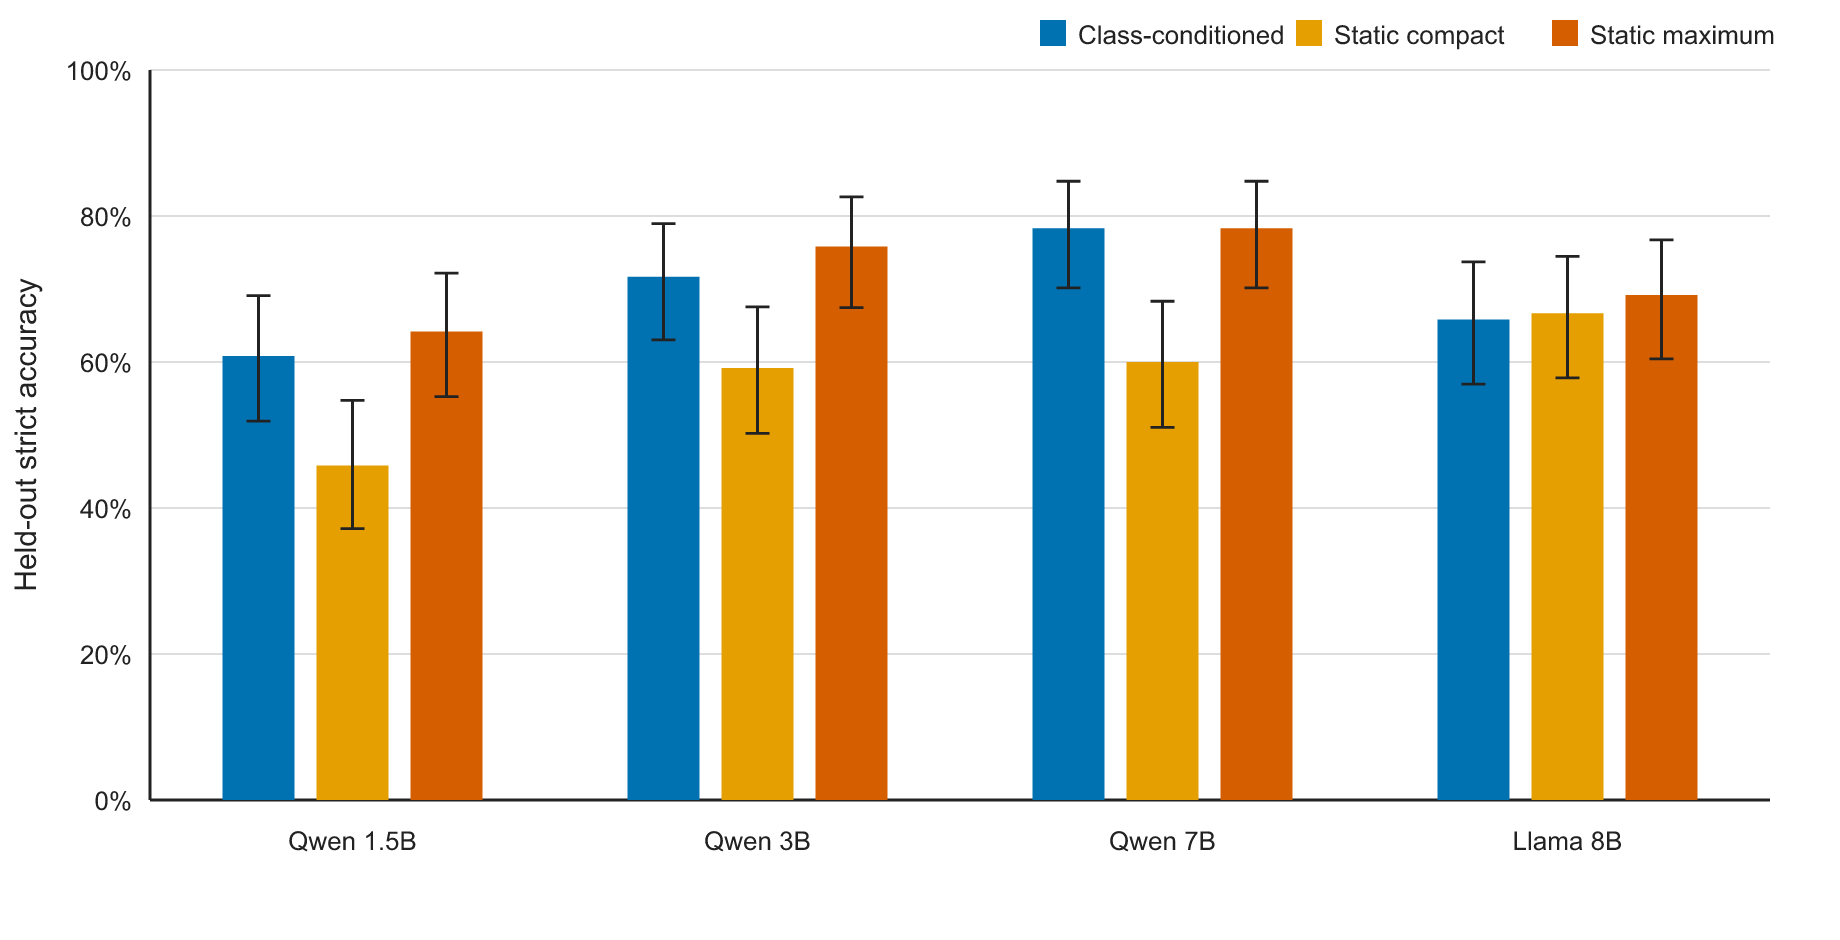
\includegraphics[width=\columnwidth]{fig1_quality_models.png}
  \caption{Held-out strategy accuracy across four models; bars show Wilson 95\% intervals ($n=120$ tasks per model and strategy).}
  \label{fig:quality-models}
\end{figure}

For Qwen2.5--3B, calibration selects standard--16 for direct readings and histories, and extended--24 for logs. The resulting held-out accuracy is 71.7\%, while maximum context reaches 75.8\%. This gap is important: the allocator uses only calibration labels, and a finite calibration corpus can choose a configuration whose held-out utility is lower than a simple static alternative.

\subsection{Main Live Mosquitto--LLM Matrix}

Table~\ref{tab:live-main} reports the 100 main runs. Under Poisson input, guarded control obtains $2.655\pm0.094$ correct on-time results/s versus $2.590\pm0.085$/s for the 3-s fixed policy. The paired gain is $0.065\pm0.059$/s (exact $p=0.0234$). It reduces expiry by $6.56\pm1.36$ percentage points ($p=0.00195$), but blocking rises by $3.74\pm1.42$ points ($p=0.00391$). The analytical deadline nearly eliminates blocking, yet its 19.6\% expiry lowers goodput to 2.343/s; low blocking alone is therefore not evidence of useful completion.

\begin{table*}[t]
\centering
\caption{Main Live Matrix: Mean $\pm$ 95\% Half-Width (Ten Paired 120-s Runs per Row)}
\label{tab:live-main}
\small
\begin{tabular}{@{}llrrr@{}}
\toprule
Traffic & Policy & Blocking (\%) & Expiry/admitted (\%) & Correct goodput (s$^{-1}$) \\
\midrule
Poisson & Fixed & $1.16\pm0.55$ & $10.20\pm2.03$ & $2.590\pm0.085$ \\
Poisson & Analytical & $0.04\pm0.10$ & $19.62\pm1.79$ & $2.343\pm0.055$ \\
Poisson & Calibrated & $7.09\pm3.39$ & $2.02\pm1.20$ & $2.647\pm0.105$ \\
Poisson & Adaptive & $5.04\pm1.64$ & $4.40\pm2.52$ & $2.634\pm0.096$ \\
Poisson & Guarded (\method{}) & $4.90\pm1.63$ & $3.64\pm1.76$ & $2.655\pm0.094$ \\
\midrule
MMPP & Fixed & $27.48\pm2.74$ & $10.24\pm2.10$ & $2.088\pm0.210$ \\
MMPP & Analytical & $16.13\pm2.50$ & $44.30\pm7.21$ & $1.473\pm0.096$ \\
MMPP & Calibrated & $30.73\pm2.78$ & $4.10\pm3.37$ & $2.115\pm0.198$ \\
MMPP & Adaptive & $21.44\pm2.32$ & $31.18\pm11.69$ & $1.685\pm0.111$ \\
MMPP & Guarded (\method{}) & $29.36\pm2.72$ & $19.88\pm6.55$ & $1.820\pm0.151$ \\
\bottomrule
\end{tabular}
\end{table*}

MMPP arrivals reverse the steady Poisson comparison. Guarded control increases blocking by $1.88\pm1.13$ points and expiry by $9.64\pm5.62$ points relative to fixed (both $p=0.00781$), while goodput decreases by $0.268\pm0.149$/s ($p=0.00391$). Calibrated feedforward has the largest mean MMPP goodput, 2.115/s, but its paired difference from fixed is only 0.027/s ($p=0.254$). The live evidence therefore does not support a traffic-independent superiority claim. The Erlang feedforward is useful in its local Poisson regime; within-epoch bursts violate the arrival approximation and fill capacity before mean-rate feedback can respond.

\begin{figure}[t]
  \centering
  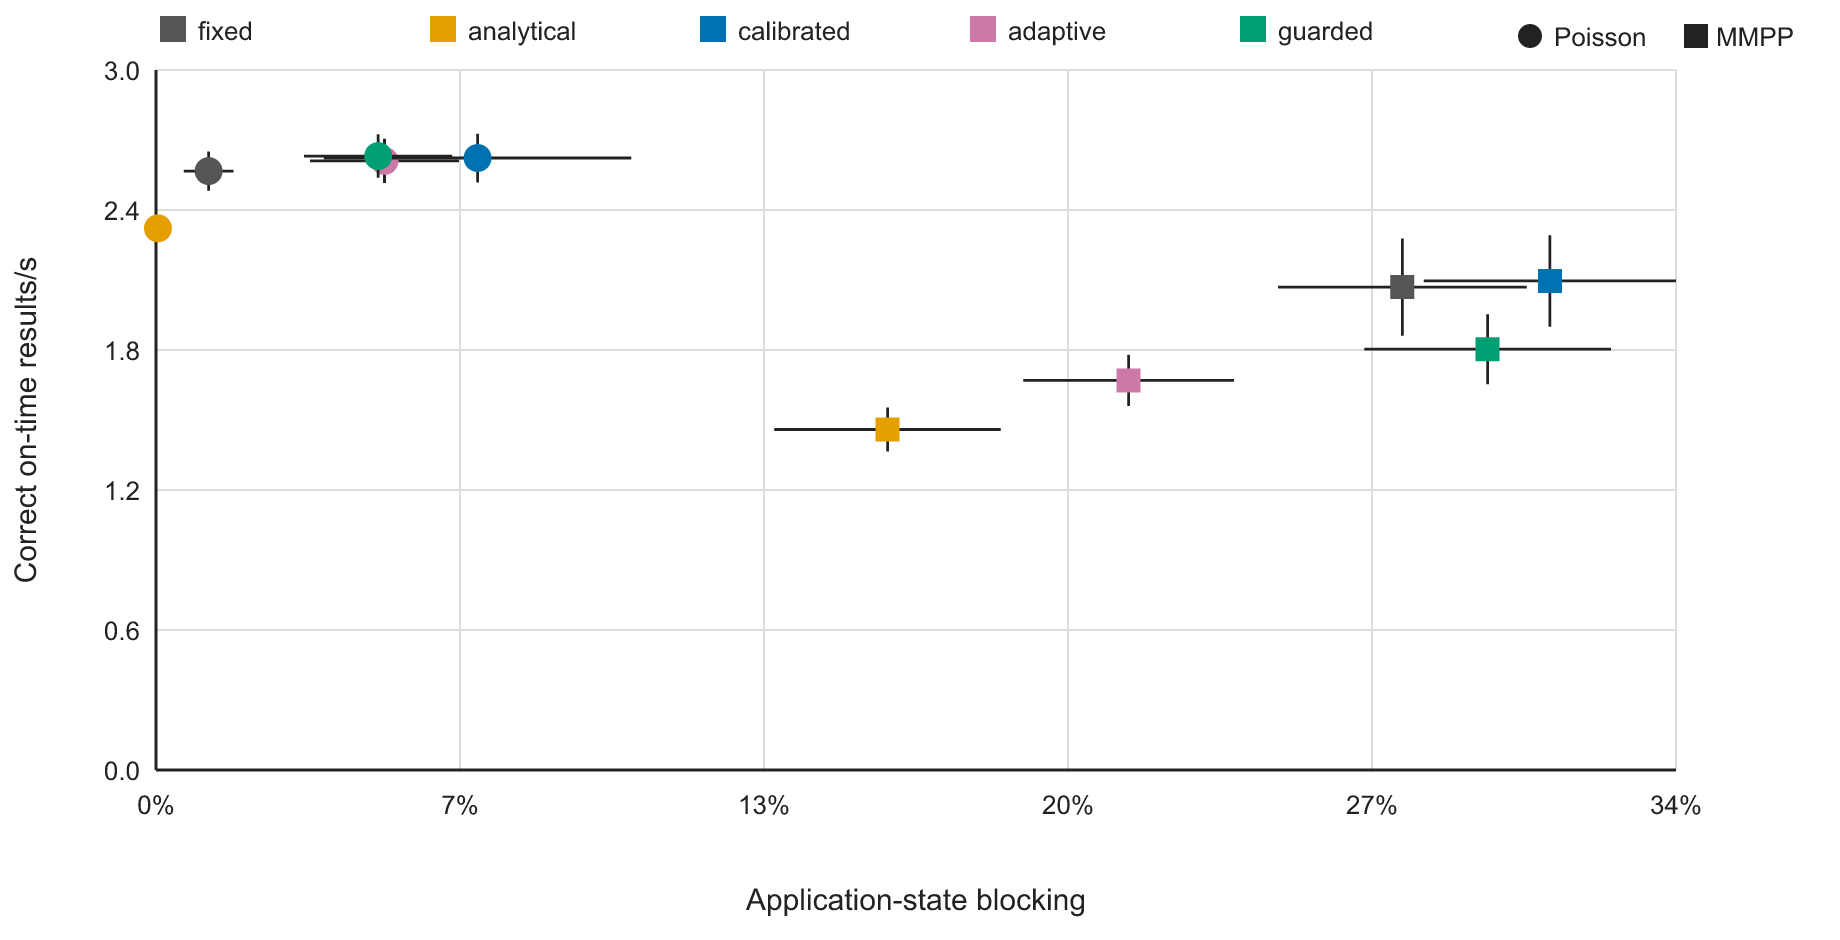
\includegraphics[width=\columnwidth]{fig2_live_tradeoff.png}
  \caption{Live blocking--goodput trade-off. Circles denote Poisson and squares MMPP; horizontal and vertical bars are 95\% intervals across ten runs.}
  \label{fig:live-tradeoff}
\end{figure}

Across all 430 selected runs, mean per-run PUBACK p95 is 1.73~ms (range 1.36--2.66~ms). By contrast, main-matrix application p95 spans means of 0.657--5.461~s across policy/traffic cells. Fast PUBACK consequently says that Mosquitto accepted protocol delivery; it does not say that an admitted inference completed before its application deadline. The measured p99 difference between end-to-end time and subscriber wall time is generally tens of milliseconds, supporting the explicit 50-ms messaging/event-loop reserve in~\eqref{eq:floors} without an arbitrary GPU/CPU multiplier.

\subsection{Fixed-Deadline Sweep and Local Stability}

The Poisson sweep compares fixed $D\in\{1,2,3,5,8\}$~s with guarded control using ten paired 60-s runs per variant. Table~\ref{tab:deadline-sweep} exposes the fixed-policy frontier: a longer deadline increases blocking but lets more admitted jobs finish. The 8-s fixed setting has the largest mean goodput, $2.755\pm0.105$/s, and is therefore the fixed comparator used in the drift study. Guarded goodput is $2.727\pm0.130$/s; its paired difference from fixed--8 is $-0.028\pm0.051$/s ($p=0.281$). Its blocking difference is $-0.41\pm0.80$ points ($p=0.375$), and expiry difference is $+1.65\pm1.76$ points ($p=0.0625$). Under stationary Poisson input, a well-tuned fixed deadline is thus competitive.

\begin{table}[t]
\centering
\caption{Poisson Deadline Sweep (Ten Paired Runs)}
\label{tab:deadline-sweep}
\small
\begin{tabular}{@{}lrrr@{}}
\toprule
Policy & Blocking (\%) & Expiry (\%) & Goodput/s \\
\midrule
Fixed--1 s & $0.04\pm0.10$ & $13.05\pm3.02$ & $2.597\pm0.123$ \\
Fixed--2 s & $0.32\pm0.35$ & $10.87\pm3.35$ & $2.645\pm0.129$ \\
Fixed--3 s & $1.12\pm0.80$ & $8.83\pm3.15$ & $2.670\pm0.127$ \\
Fixed--5 s & $2.88\pm1.73$ & $4.82\pm2.52$ & $2.737\pm0.135$ \\
Fixed--8 s & $5.13\pm3.21$ & $1.15\pm0.83$ & $2.755\pm0.105$ \\
Guarded & $4.72\pm2.80$ & $2.80\pm2.11$ & $2.727\pm0.130$ \\
\bottomrule
\end{tabular}
\end{table}

\begin{figure}[t]
  \centering
  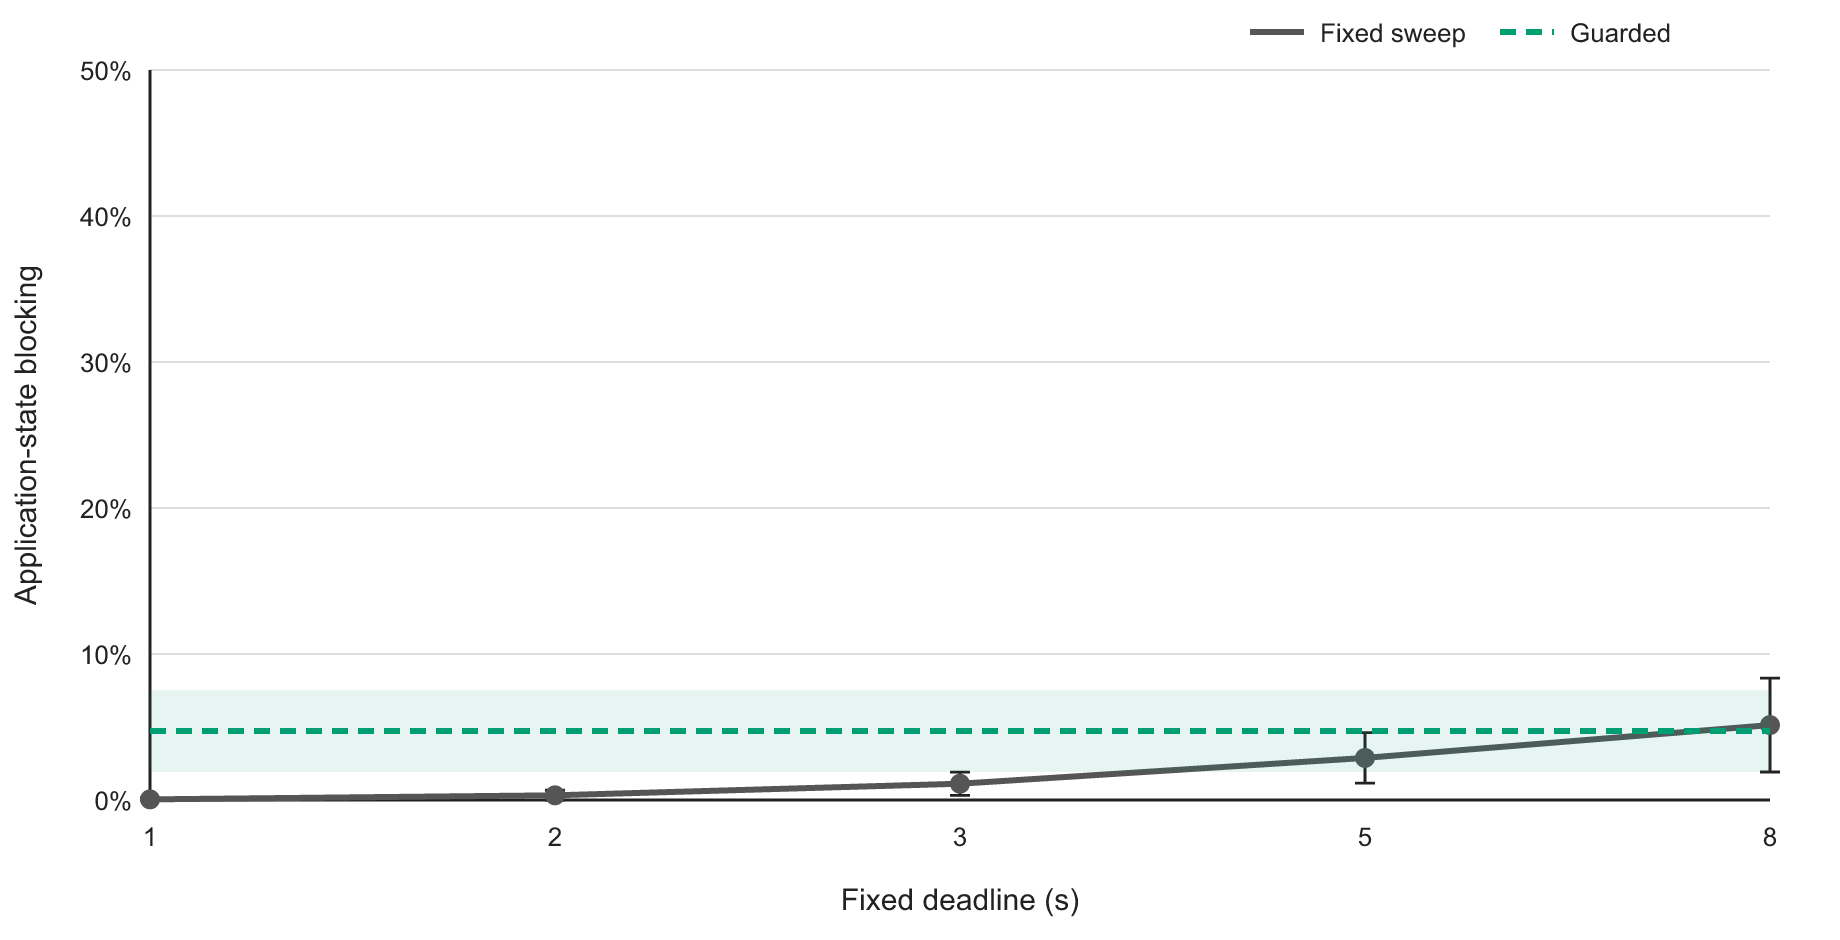
\includegraphics[width=\columnwidth]{fig3_deadline_sweep.png}
  \caption{Fixed-deadline blocking with 95\% intervals. The shaded band is the guarded mean interval.}
  \label{fig:deadline-sweep}
\end{figure}

A finite-difference fit to the log-deadline blocking response near the 5\% target gives $g=0.04095$. With $a=0.7$ and $\eta=1.5$, the left side of~\eqref{eq:stability-condition} is $\eta(1-a)g=0.0184$, well below $2(1+a)=3.4$. The implemented gain therefore satisfies Proposition~1's local condition at this operating point. This is a local feedback result, not a guarantee under MMPP input, clipping, or an infeasible capacity target.

\subsection{Live Allocation Baselines}

Figure~\ref{fig:allocator} compares four allocators using a Latin-square order over ten matched Poisson seeds. Quality-aware selection raises on-time strict accuracy from $60.75\pm1.00$\% for static compact to $73.08\pm0.98$\%; the paired gain is $12.33\pm1.30$ points ($p=0.00195$). Goodput increases from $2.417\pm0.091$ to $2.697\pm0.144$/s ($p=0.00391$). This gain is not free: blocking increases by $3.95\pm2.10$ points and expiry by $3.44\pm2.40$ points (both $p=0.00391$).

Static maximum context and token-max are stronger here. Their accuracies are $75.88\pm0.95$\% and $76.10\pm0.94$\%, with goodputs $2.962\pm0.104$ and $2.985\pm0.121$/s. Quality-aware selection is lower by 2.80 and 3.02 accuracy points, respectively, and by 0.265 and 0.288 results/s (all paired $p=0.00195$). The ordering places quality-aware selection between the compact latency-oriented rule and the stronger maximum-budget rules on this model and corpus.

\begin{figure}[t]
  \centering
  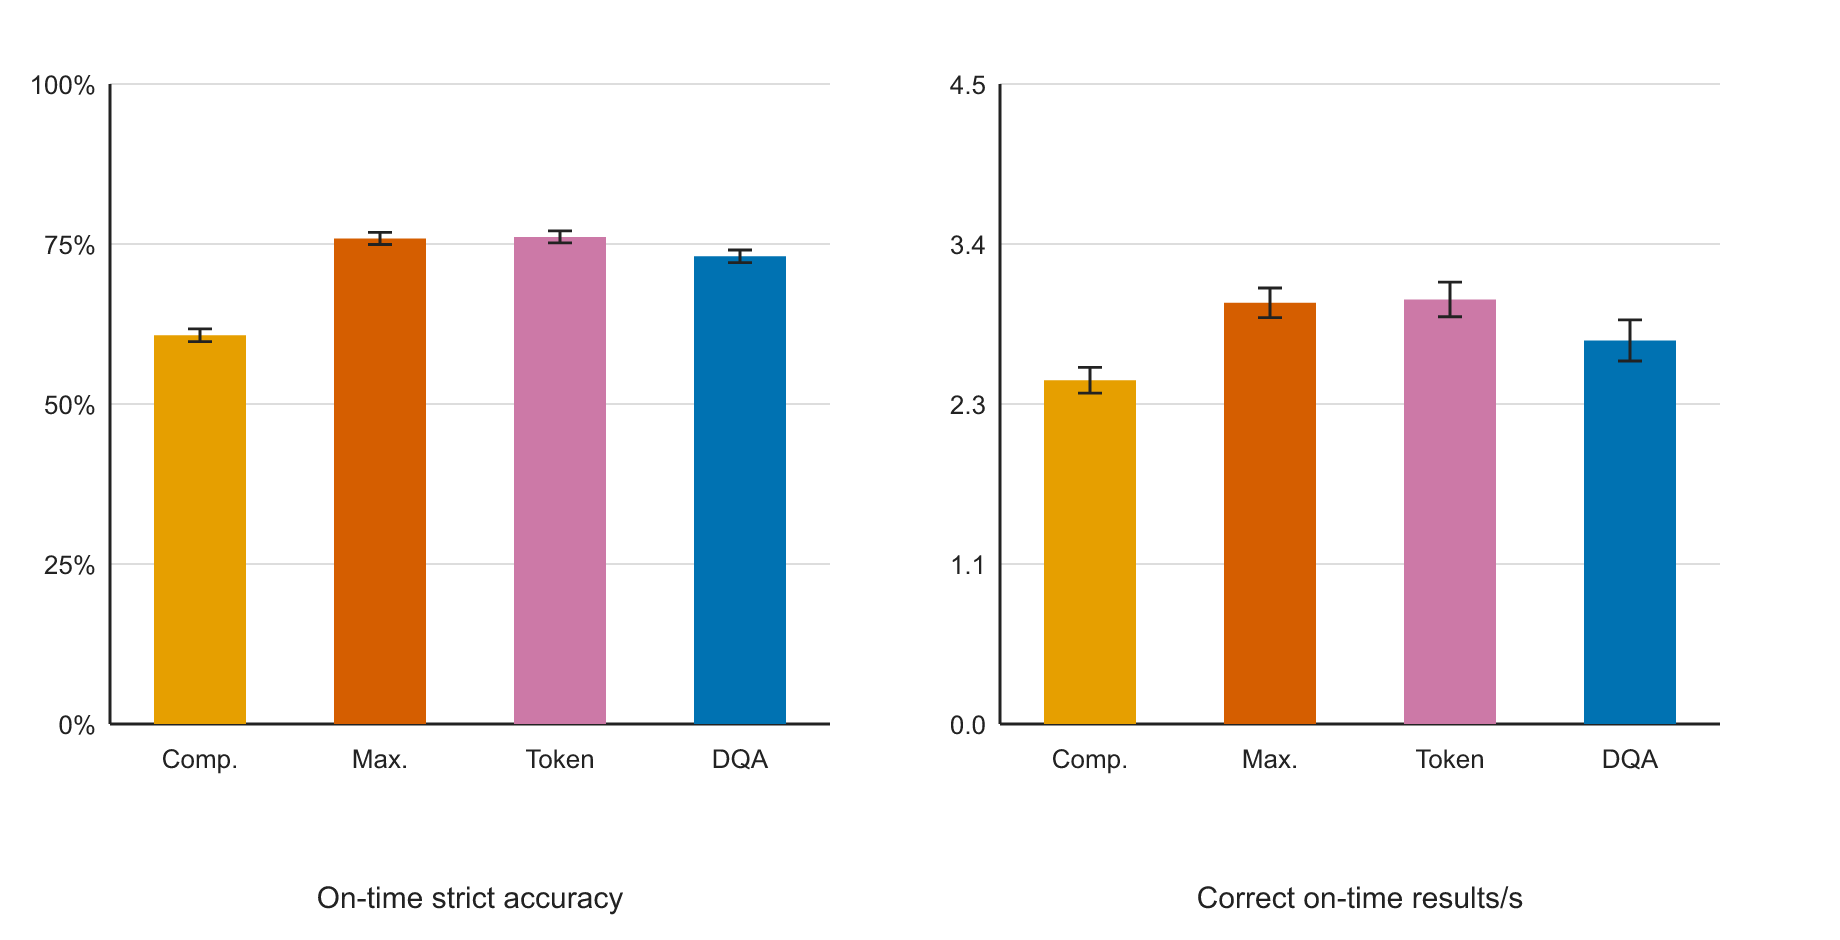
\includegraphics[width=\columnwidth]{fig4_allocator.png}
  \caption{Matched live allocator study. Error bars are 95\% intervals across ten runs. ``Max.'' is static extended--48; ``Token'' maximizes feasible prompt-plus-output budget.}
  \label{fig:allocator}
\end{figure}

\subsection{Model-Service Drift}

The drift workload uses 60~s with a Poisson rate step from 2/s to 6/s at 30~s and switches the service model from Qwen2.5--3B to 7B at the same instant. Fixed uses the sweep-selected 8-s deadline. Figure~\ref{fig:drift} summarizes ten paired seeds. Guarded control lowers blocking from $33.38\pm4.76$\% to $23.77\pm3.22$\%, a paired change of $-9.61\pm2.91$ points ($p=0.00195$). Expiry falls from $17.63\pm2.74$\% to $14.32\pm3.05$\% ($-3.31\pm2.51$ points, $p=0.0215$), and goodput rises from $1.605\pm0.116$ to $1.922\pm0.072$/s ($+0.317\pm0.124$/s, $p=0.00195$). Accuracy does not change significantly ($p=0.643$). Guarded control reroutes $7.4\pm2.76$ jobs per run, whereas fixed does not reroute.

This result locates the controller's practical advantage: not a stationary setting for which a fixed deadline can be tuned after the fact, but a service distribution and arrival rate that move away from that tuning point. The common 8-s maximum is used in every live study; the class floor adapts through measured p95 service, FIFO work ahead, and the 50-ms reserve rather than class-specific constants.

\begin{figure}[t]
  \centering
  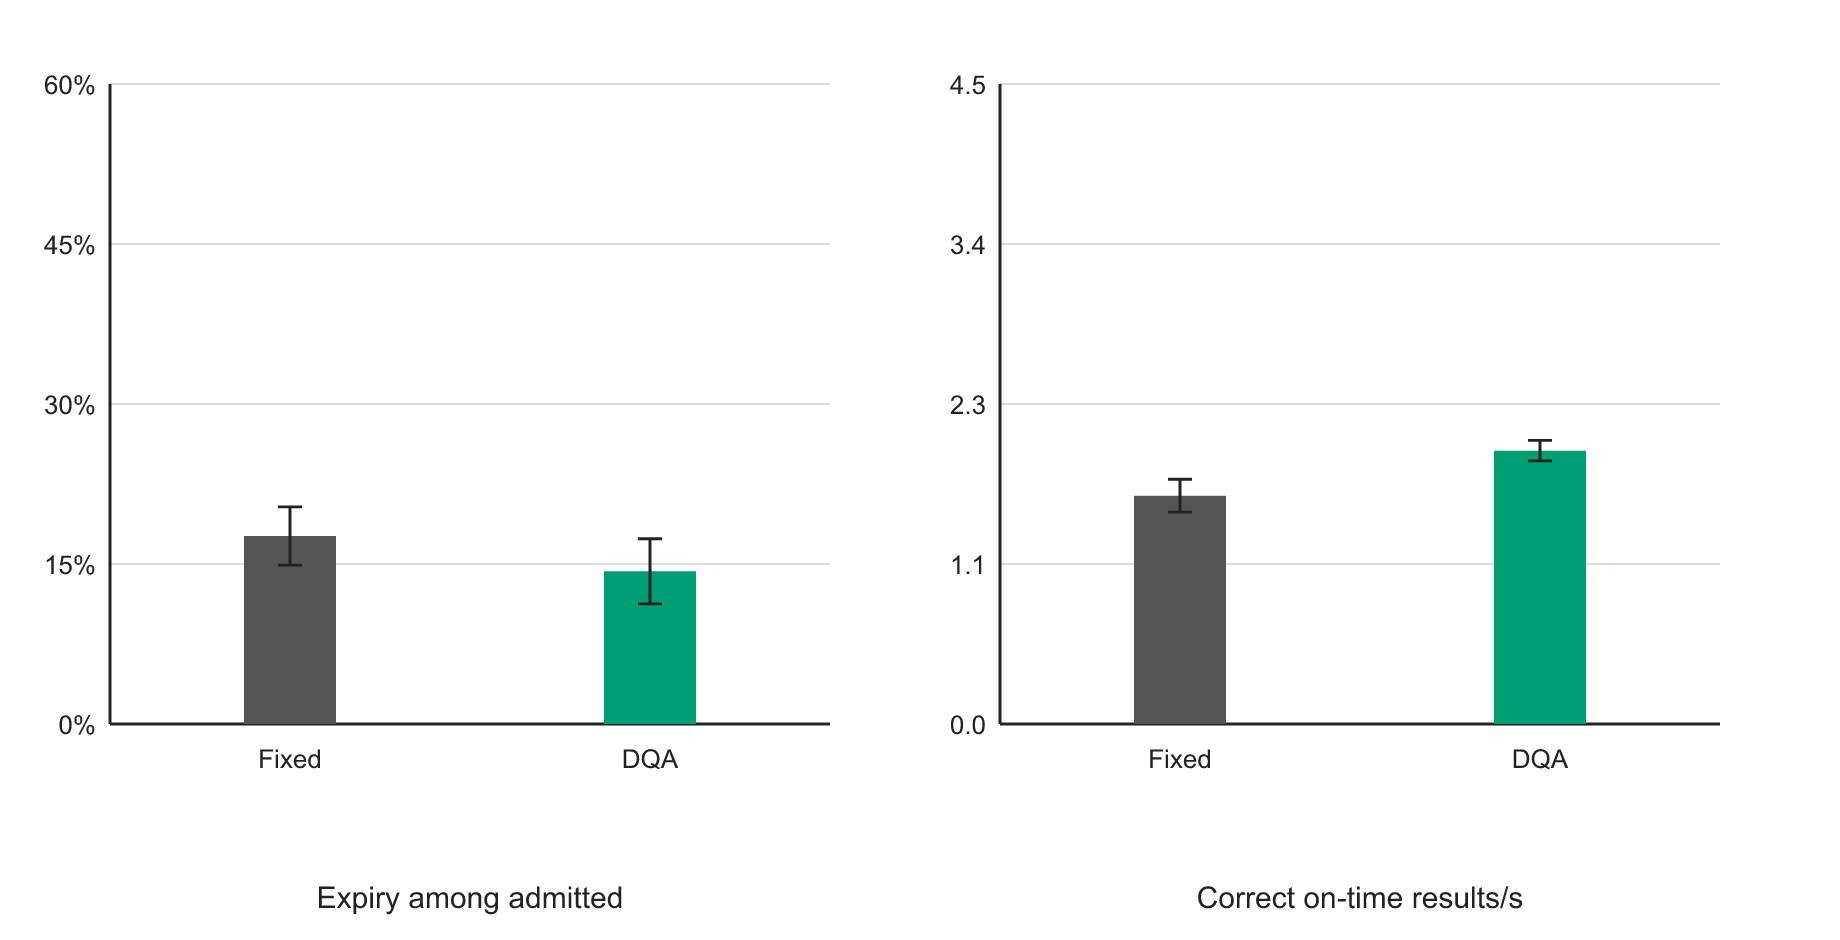
\includegraphics[width=\columnwidth]{fig5_drift.png}
  \caption{Fixed--8 versus guarded control during simultaneous rate and model-service drift; error bars are 95\% intervals.}
  \label{fig:drift}
\end{figure}

\subsection{Comparison with Conventional Admission Control}

Table~\ref{tab:standard-baselines} and Fig.~\ref{fig:standard-baselines} compare \method{} with the four reference rules defined in Section~\ref{sec:controller}. Each row summarizes ten paired seeds. Under Poisson input, \method{} lowers blocking by 6.64 points relative to B1 ($p=0.00195$) while its 0.090/s goodput increase is not significant ($p=0.0684$). Its goodput advantages over B2 and B3 are 0.455/s and 0.837/s (both $p=0.00195$). Against FIFO without proactive admission, it lowers blocking by 4.18 points and gains 0.113/s (both $p=0.00195$), with nearly identical expiry. The lower blocking relative to B1 is accompanied by more post-admission expiry, showing that early rejection and timely completion are distinct outcomes.

\begin{table*}[t]
\centering
\caption{\method{} and Conventional Admission Baselines: Mean $\pm$ 95\% Half-Width (Ten Paired Runs per Row)}
\label{tab:standard-baselines}
\small
\begin{tabular}{@{}llrrr@{}}
\toprule
Scenario & Method & Blocking (\%) & Expiry/admitted (\%) & Correct goodput (s$^{-1}$) \\
\midrule
Poisson & \method{} & $4.90\pm1.63$ & $3.64\pm1.76$ & $2.655\pm0.094$ \\
 & B1: occupancy threshold & $11.54\pm3.66$ & $0.72\pm1.05$ & $2.565\pm0.142$ \\
 & B2: static reservation & $22.56\pm9.12$ & $2.59\pm1.96$ & $2.200\pm0.260$ \\
 & B3: threshold + reservation & $36.69\pm7.58$ & $0.56\pm0.44$ & $1.818\pm0.206$ \\
 & FIFO: no proactive admission & $9.08\pm3.41$ & $3.62\pm1.66$ & $2.542\pm0.138$ \\
\midrule
MMPP & \method{} & $29.36\pm2.72$ & $19.88\pm6.55$ & $1.820\pm0.151$ \\
 & B1: occupancy threshold & $37.02\pm4.89$ & $0.16\pm0.15$ & $2.006\pm0.161$ \\
 & B2: static reservation & $52.11\pm6.66$ & $4.69\pm2.52$ & $1.437\pm0.145$ \\
 & B3: threshold + reservation & $61.41\pm4.72$ & $1.62\pm1.38$ & $1.181\pm0.085$ \\
 & FIFO: no proactive admission & $32.52\pm3.90$ & $1.60\pm0.96$ & $2.122\pm0.243$ \\
\midrule
Rate/model drift & \method{} & $23.77\pm3.22$ & $14.32\pm3.05$ & $1.922\pm0.072$ \\
 & B1: occupancy threshold & $43.11\pm4.71$ & $16.11\pm2.71$ & $1.395\pm0.132$ \\
 & B2: static reservation & $55.70\pm3.89$ & $29.83\pm5.31$ & $0.880\pm0.140$ \\
 & B3: threshold + reservation & $67.02\pm3.73$ & $31.71\pm5.70$ & $0.648\pm0.118$ \\
 & FIFO: no proactive admission & $32.21\pm4.12$ & $17.14\pm2.65$ & $1.655\pm0.121$ \\
\bottomrule
\end{tabular}
\end{table*}

Under MMPP input, \method{} again lowers blocking relative to B1 by 7.66 points ($p=0.00195$), but B1 nearly eliminates expiry and obtains 0.186/s more goodput ($p=0.0215$). FIFO has 3.17 points more blocking ($p=0.00195$), 18.28 points less expiry ($p=0.00195$), and 0.302/s more goodput ($p=0.00977$) than \method{}. In contrast, \method{} exceeds B2 and B3 by 0.383/s ($p=0.00391$) and 0.639/s ($p=0.00195$). This is a genuine operating-point trade-off: B1 rejects more requests before execution, while FIFO and \method{} admit more work but retain it for different durations when a burst outruns the mean-rate controller.

The drift condition gives the clearest separation. Relative to B1, \method{} reduces blocking by 19.34 points and increases goodput by 0.527/s (both $p=0.00195$); the 1.80-point expiry reduction is not significant ($p=0.217$). Relative to B2 and B3, the goodput gains are 1.042/s and 1.273/s, while blocking falls by 31.92 and 43.25 points and expiry by 15.51 and 17.40 points (all $p=0.00195$). Relative to FIFO, \method{} reduces blocking by 8.44 points, expiry by 2.83 points, and gains 0.267/s ($p=0.00195$, $0.0313$, and $0.00195$, respectively). Neither a static guard rule nor unrestricted FIFO admission follows the simultaneous change in offered rate and service time.

\begin{figure*}[t]
  \centering
  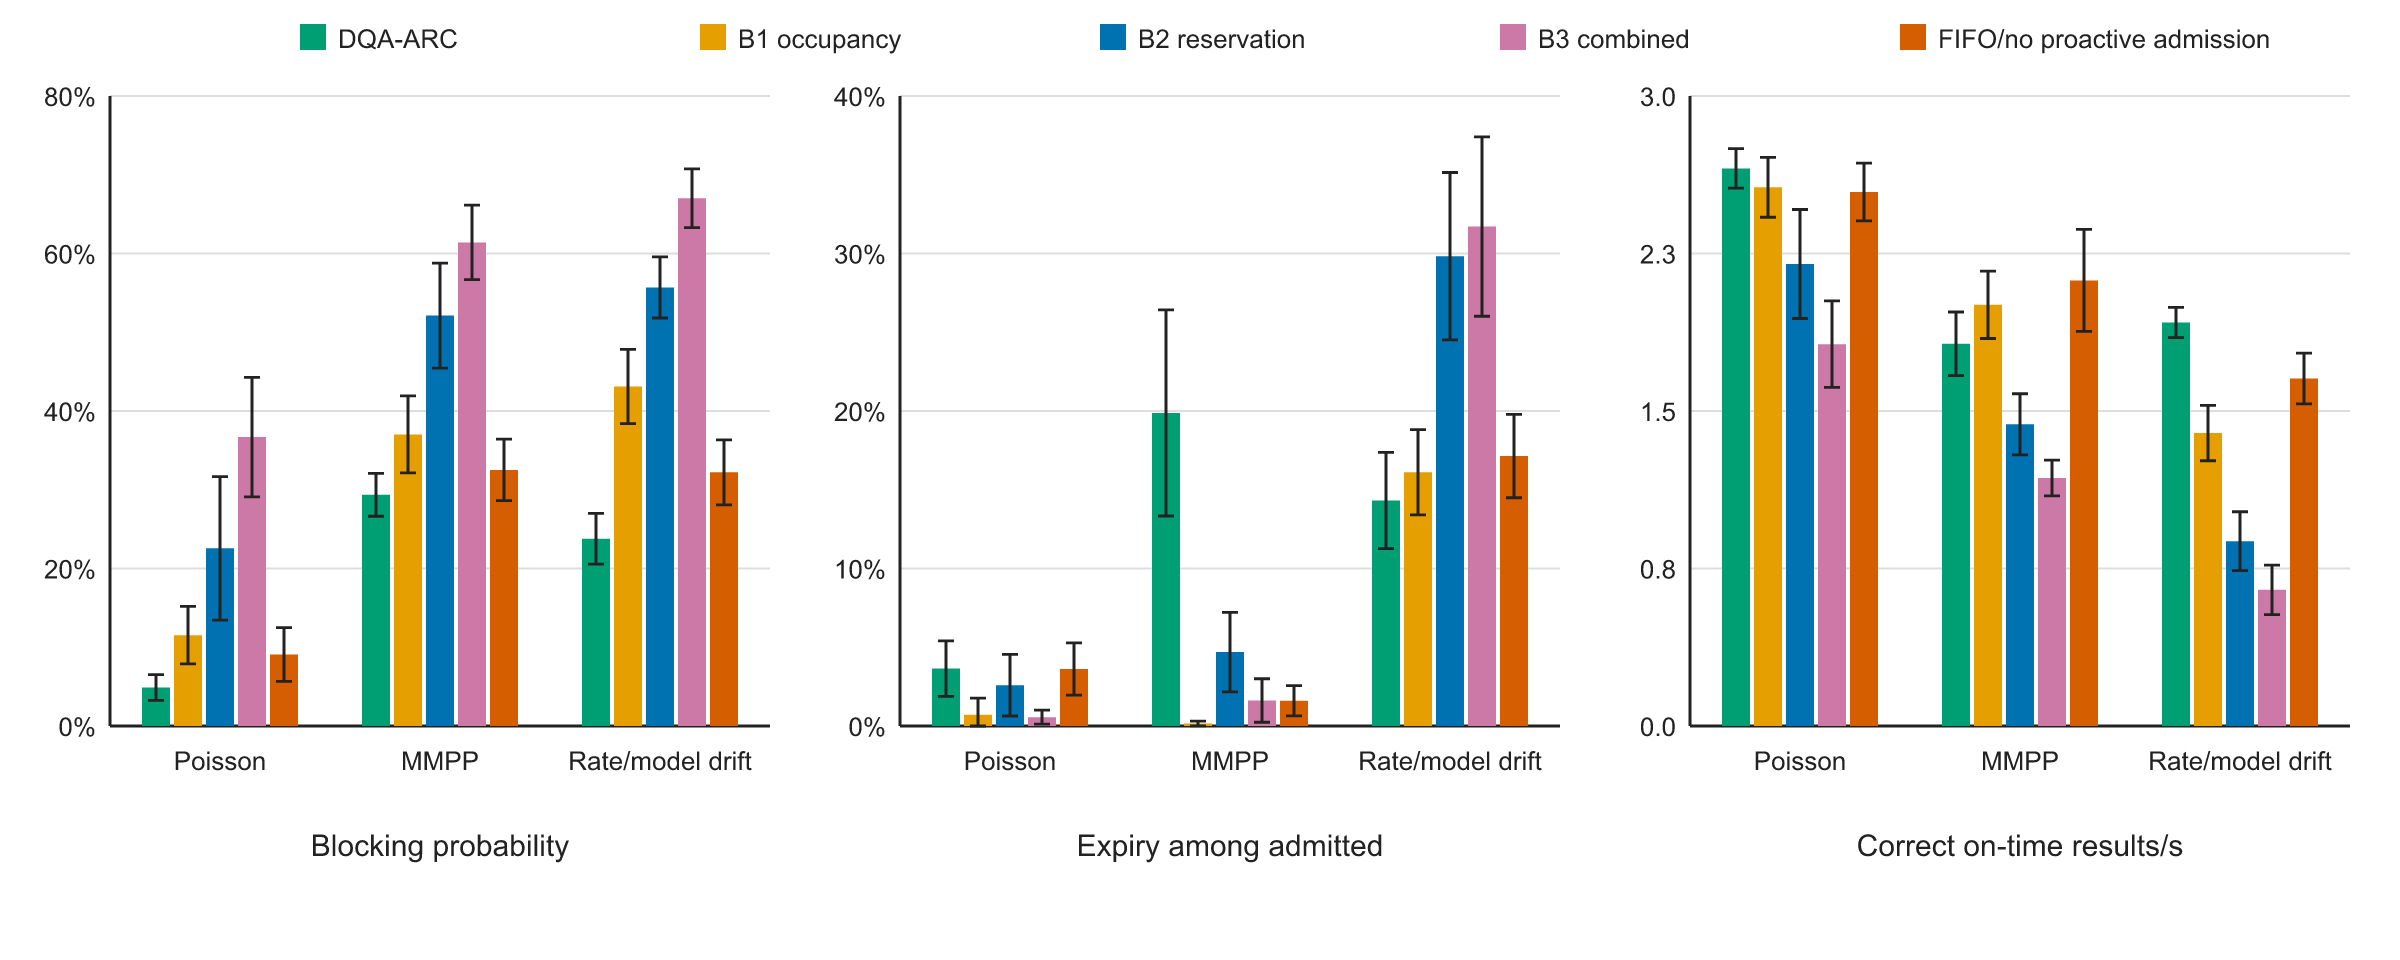
\includegraphics[width=0.99\textwidth]{fig7_standard_baselines.png}
  \caption{Live comparison with reference admission controls. Bars show means and 95\% intervals across ten paired seeds. B1 uses an occupancy threshold, B2 static class reservation, B3 their combination, and FIFO admits until the common hard capacity without proactive shedding.}
  \label{fig:standard-baselines}
\end{figure*}

\subsection{Occupancy-Threshold Sensitivity}

Table~\ref{tab:threshold-sweep} evaluates the prespecified B1 rule over $\theta\in\{4,5,6,7\}$ without replacing the headline $\theta=6$ setting. Under Poisson input, increasing $\theta$ moves B1 along the expected admission frontier: blocking falls from $19.31\pm4.82$\% to $9.10\pm3.47$\%, while goodput rises from $2.344\pm0.189$/s to $2.623\pm0.088$/s. At $\theta=7$, the goodput difference from \method{} is only $0.032\pm0.054$/s (Holm-adjusted $p=0.256$), but \method{} still blocks 4.21 percentage points less ($p_{\mathrm{Holm}}=0.00781$). Thus, a less conservative threshold can close the stationary-Poisson goodput gap but not the blocking gap.

MMPP traffic reverses the goodput ordering. B1 at $\theta=7$ obtains $2.099\pm0.201$/s versus \method{}'s $1.820\pm0.151$/s, a paired B1 advantage of $0.279\pm0.134$/s ($p_{\mathrm{Holm}}=0.0156$). It does so with $33.54\pm4.20$\% blocking versus 29.36\% for \method{}, and only 0.57\% expiry versus 19.88\%. The threshold converts burst pressure into early rejection; no tested value jointly matches \method{}'s lower blocking and B1's lower expiry.

The drift result is robust to the full range. The closest B1 point, $\theta=7$, reaches $1.515\pm0.150$/s, leaving a \method{} advantage of $0.407\pm0.148$/s, while its blocking is 13.85 points higher (both $p_{\mathrm{Holm}}=0.00781$). The goodput gaps at $\theta=4,5,6$ are 0.815, 0.635, and 0.527/s, respectively, and all four Holm-adjusted comparisons remain significant. Hence a tested static threshold does not close the simultaneous rate/model-drift gap.

\begin{table*}[t]
\centering
\caption{B1 Occupancy-Threshold Sensitivity: Mean $\pm$ 95\% Half-Width (Ten Paired Runs per Row)}
\label{tab:threshold-sweep}
\small
\begin{tabular}{@{}llrrr@{}}
\toprule
Scenario & Method & Blocking (\%) & Expiry/admitted (\%) & Correct goodput (s$^{-1}$) \\
\midrule
Poisson & \method{} & $4.90\pm1.63$ & $3.64\pm1.76$ & $2.655\pm0.094$ \\
 & B1, $\theta=4$ & $19.31\pm4.82$ & $0.40\pm0.85$ & $2.344\pm0.189$ \\
 & B1, $\theta=5$ & $13.95\pm3.32$ & $0.05\pm0.08$ & $2.502\pm0.107$ \\
 & B1, $\theta=6$ & $11.54\pm3.66$ & $0.72\pm1.05$ & $2.565\pm0.142$ \\
 & B1, $\theta=7$ & $9.10\pm3.47$ & $0.80\pm0.52$ & $2.623\pm0.088$ \\
\midrule
MMPP & \method{} & $29.36\pm2.72$ & $19.88\pm6.55$ & $1.820\pm0.151$ \\
 & B1, $\theta=4$ & $42.52\pm4.40$ & $0.00\pm0.00$ & $1.837\pm0.146$ \\
 & B1, $\theta=5$ & $39.28\pm5.05$ & $0.06\pm0.09$ & $1.943\pm0.203$ \\
 & B1, $\theta=6$ & $37.02\pm4.89$ & $0.16\pm0.15$ & $2.006\pm0.161$ \\
 & B1, $\theta=7$ & $33.54\pm4.20$ & $0.57\pm0.40$ & $2.099\pm0.201$ \\
\midrule
Rate/model drift & \method{} & $23.77\pm3.22$ & $14.32\pm3.05$ & $1.922\pm0.072$ \\
 & B1, $\theta=4$ & $56.01\pm6.30$ & $15.18\pm3.92$ & $1.107\pm0.185$ \\
 & B1, $\theta=5$ & $48.11\pm4.68$ & $15.98\pm2.62$ & $1.287\pm0.140$ \\
 & B1, $\theta=6$ & $43.11\pm4.71$ & $16.11\pm2.71$ & $1.395\pm0.132$ \\
 & B1, $\theta=7$ & $37.62\pm4.63$ & $18.23\pm3.34$ & $1.515\pm0.150$ \\
\bottomrule
\end{tabular}
\end{table*}

\begin{figure*}[t]
  \centering
  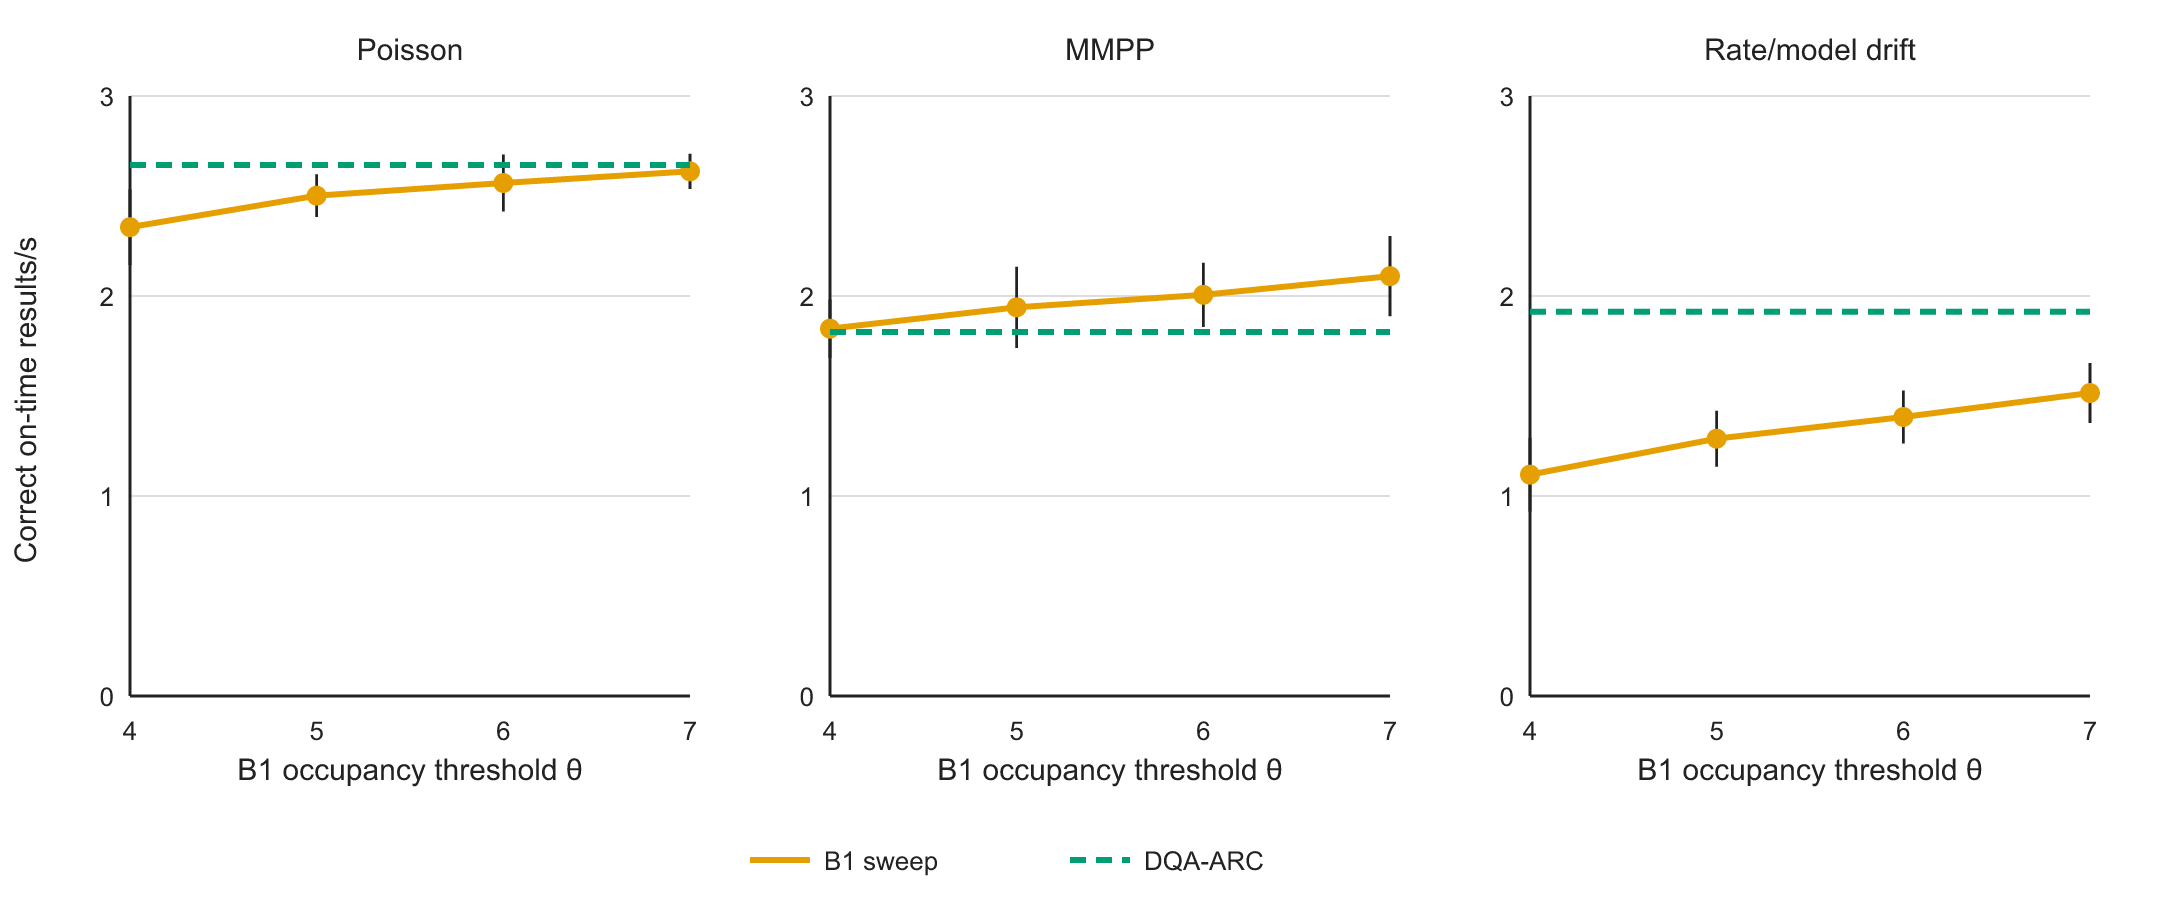
\includegraphics[width=0.92\textwidth]{fig8_b1_threshold_sweep.png}
  \caption{B1 threshold sensitivity for correct on-time goodput. Points and bars show B1 means and 95\% intervals; dashed lines are \method{} means in the corresponding scenarios.}
  \label{fig:threshold-sweep}
\end{figure*}

Table~\ref{tab:class-baselines} exposes the mechanisms by preferred class. B2 reduces CPU-preferred blocking relative to B1 under Poisson (4.3\% versus 10.9\%) and MMPP (21.1\% versus 36.3\%), but increases GPU-preferred blocking to 27.7\% and 60.7\%. B3 strengthens this trade-off. Under drift, B2 and \method{} have similar CPU-preferred blocking (22.6\% and 22.9\%), yet B2's CPU expiry is 79.1\% versus 63.1\% and its CPU goodput is 0.085/s versus 0.175/s. FIFO retains 0.077/s CPU goodput under drift, compared with 0.175/s for \method{}, because 78.6\% of its admitted CPU-preferred work expires. Reservation alone protects admission opportunity, and FIFO alone avoids reserved idle capacity, but neither ensures timely completion of the protected slow class.

\begin{table*}[t]
\centering
\caption{Preferred-Class Blocking/Correct-Goodput (\% / s$^{-1}$)}
\label{tab:class-baselines}
\scriptsize
\begin{tabular}{@{}llrrrrr@{}}
\toprule
Scenario & Preferred class & \method{} & B1 occupancy & B2 reservation & B3 combined & FIFO \\
\midrule
Poisson & GPU & $4.9/2.176$ & $11.6/2.020$ & $27.7/1.647$ & $44.9/1.248$ & $9.1/2.065$ \\
 & CPU & $5.0/0.479$ & $10.9/0.545$ & $4.3/0.552$ & $7.6/0.571$ & $8.8/0.478$ \\
MMPP & GPU & $29.1/1.522$ & $37.2/1.579$ & $60.7/0.972$ & $70.7/0.720$ & $32.0/1.712$ \\
 & CPU & $30.3/0.298$ & $36.3/0.427$ & $21.1/0.464$ & $27.7/0.461$ & $34.3/0.410$ \\
Rate/model drift & GPU & $24.1/1.747$ & $44.2/1.302$ & $64.6/0.795$ & $75.9/0.555$ & $32.6/1.578$ \\
 & CPU & $22.9/0.175$ & $39.3/0.093$ & $22.6/0.085$ & $34.2/0.093$ & $30.5/0.077$ \\
\bottomrule
\end{tabular}
\end{table*}

\subsection{Burst-Robust Replay}

The burst-guarded variant places a token bucket before application-state admission. Tokens accrue at the target mean rate; a request may wait at most 2~s for a token, after which it is counted as a shaper drop. Figure~\ref{fig:burst-guard} reports MMPP rate 4/s with 20\% CPU preference. At capacities 4, 8, and 12, guarded broker blocking is $31.87\pm0.56$\%, $17.54\pm0.49$\%, and $9.36\pm0.45$\%. The token bucket reduces broker blocking to $0.97\pm0.12$\%, $0.005\pm0.010$\%, and zero, respectively.

Broker blocking alone gives the wrong conclusion. Token-bucket total admission loss is $35.40\pm0.75$\%, $34.86\pm0.65$\%, and $34.72\pm0.87$\% because requests are discarded at the shaper; mean shaping delay is about $0.86\pm0.02$~s. At capacity 12, guarded goodput is $2.555\pm0.052$/s, whereas burst-guarded goodput is $1.836\pm0.025$/s. The implemented shaper protects broker state but fails to improve end-to-end admission utility for this MMPP. This negative boundary result motivates state estimation or reservation that can distinguish a transient burst from sustained overload rather than a fixed-rate bucket.

\begin{figure}[t]
  \centering
  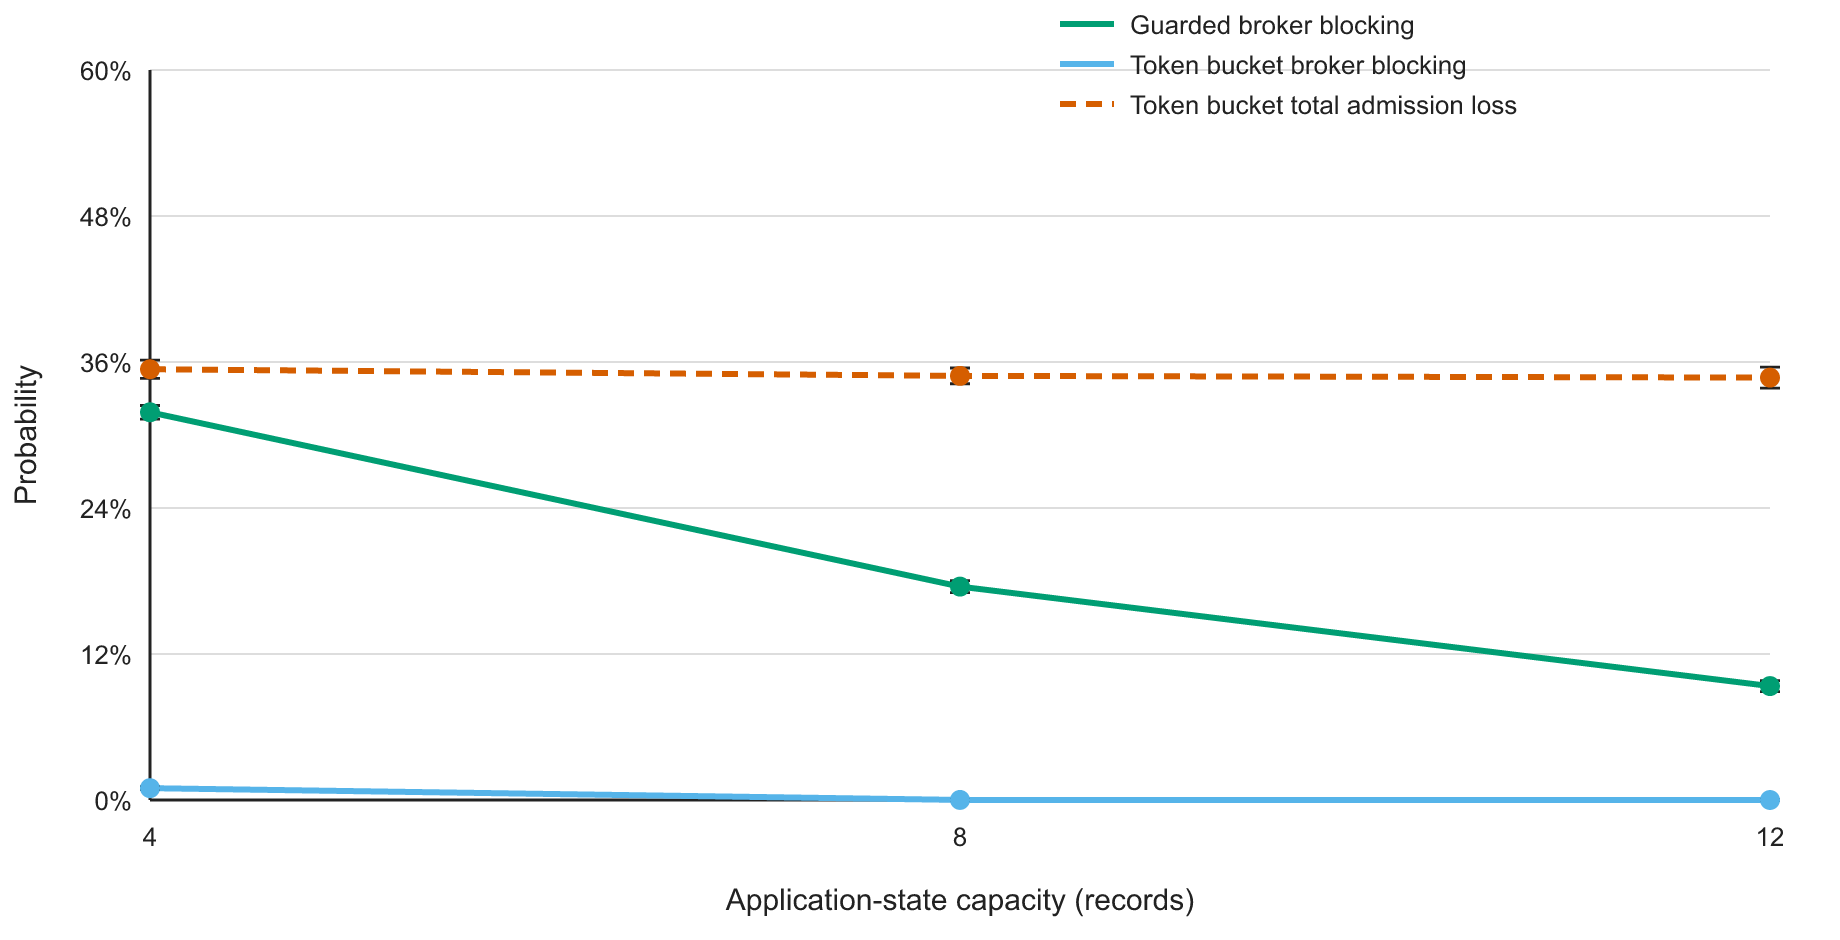
\includegraphics[width=\columnwidth]{fig6_burst_guard.png}
  \caption{MMPP replay with 95\% intervals. Token-bucket shaping nearly eliminates broker blocking, but total admission loss includes shaper drops and remains high.}
  \label{fig:burst-guard}
\end{figure}

Under Poisson rate 4/s, replay shows a different operating region: guarded blocking falls from $6.01\pm0.22$\% at capacity four to $0.393\pm0.077$\% at eight and $0.0025\pm0.0028$\% at 12, with negligible expiry. Thus, capacity eight is compatible with the 5\% target for the measured Poisson profile but not for the MMPP. The contrast is consistent with the live matrix and clarifies that mean offered load is insufficient to characterize burst feasibility.

\subsection{Answers to the Evaluation Questions}

Q1: Class-conditioned selection beats compact for the three Qwen sizes but does not universally beat maximum context or transfer unchanged to Llama. Q2: Under stationary Poisson input, guarded control slightly improves goodput over fixed while trading more blocking for less expiry; under MMPP it is worse than fixed. Q3: Against the sweep-selected fixed deadline, guarded control improves blocking, expiry, and goodput during simultaneous rate/model drift. Q4: The measured Poisson slope satisfies the stated local Jury condition, whose assumptions exclude burst mismatch. Q5: millisecond PUBACK coexists with second-scale application completion and does not certify inference success. Q6: bounded-delay token-bucket shaping protects broker capacity but relocates enough loss to the shaper that total admission utility deteriorates under the tested MMPP. Q7: \method{} provides the largest goodput under drift against B1--B3 and FIFO, and this conclusion holds across all four B1 thresholds; under MMPP, FIFO and a less restrictive B1 threshold obtain higher goodput by accepting different trade-offs between blocking and expiry.
% END INLINED sections/05_evaluation.tex
% BEGIN INLINED sections/06_discussion.tex
\section{Discussion and Limitations}
\label{sec:discussion}

\subsection{What the Analytical Model Does---and Does Not---Show}

Equation~\eqref{eq:erlang-recursion} is useful because it converts capacity and a desired loss probability into a transparent offered-load budget. It does not prove that a finite trace, an MMPP, correlated retries, or a queueing LLM subscriber will meet that probability. Similarly, numerically selecting $A$ so that $B_n(A)=\alpha$ and then plotting $B_n(A)$ is an identity, not validation. Our evidence instead comes from correlated completion, expiry, task accuracy, PUBACK timing, and blocking observed outside that equation.

The experiments also show why a single objective is hazardous. The analytical and adaptive ablations sometimes approach or beat the blocking target by setting a deadline that removes admitted state before useful work completes. A deployment must decide whether rejecting at admission, expiring after admission, or returning a lower-quality fast result has the lowest cost. \method{} currently emphasizes completion of admitted work through feasibility floors; this can raise blocking. A future formulation should optimize a weighted utility or constrained vector of blocking, expiry, quality, and class fairness rather than treating one target as sufficient.

The conventional comparators reinforce this point. An occupancy threshold is difficult to beat on simplicity and, under MMPP traffic, converts burst pressure into early rejection with little post-admission expiry. Static reservation can protect admission opportunity for the minority CPU-preferred class, but the protected jobs may still expire and their occupancy can displace many shorter GPU-preferred jobs. The combined threshold/reservation rule is therefore not automatically safer: in this workload it is conservative for the majority class without adapting to the protected class's service drift. FIFO operation at the hard capacity removes proactive shedding but exposes admitted records to the full queue. The threshold sensitivity study separates this admission trade-off from a favorable choice of one $\theta$. \method{} is most useful when service and load move together, while a fixed threshold remains a credible choice when early rejection is acceptable and the workload is persistently bursty.

\subsection{Deployment Scope}

The controller is an application-layer sidecar, not a modified Mosquitto binary. This choice improves portability and preserves MQTT conformance, but adds a process and duplicates selected request metadata. A production design could move the same state machine into a broker plugin, persistent gateway service, or replicated control plane. Crash recovery, exactly-once application effects, multi-broker correlation, authentication/authorization, TLS overhead, and adversarial correlation identifiers are outside this prototype. MQTT QoS~1 can redeliver an Application Message; a production controller must make $id_i$ admission and completion idempotent.

The experiment uses loopback networking and one physical host. It isolates broker semantics, execution-class differences, and LLM service time, but does not reproduce wireless loss, WAN delay, battery/thermal throttling, or many-device contention. In particular, a deliberately slow remote subscriber and controlled network delay/loss (for example with \texttt{tc netem}) remain external-validity tests rather than claims of this study. The CPU-only endpoint is a software-enforced execution class on the Ryzen host. The reported process memory is therefore an implementation measurement, not a general broker-overhead model.

The 240-example corpus provides exact, reproducible labels and makes conflicting context controllable, but it remains synthetic. It spans two prompt templates, four sensor domains, and direct-reading, history-dependent, and unstructured-log requests; half of the items are held out. Profiles across three Qwen2.5 sizes and Llama~3.1--8B expose model dependence, but broader domain datasets, quantizations, and human-authored logs remain necessary. Strict JSON validity is relevant to machine-to-machine IoT control, yet other applications require F1, calibration, factuality, human preference, or safety review. Quality profiles must be regenerated after any model, runtime, or policy change.

The p95 FIFO floor in~\eqref{eq:floors}, feedback gain, epoch duration, and 30\% rate limiter were engineering choices evaluated on one host. They are disclosed to enable replication but are not claimed optimal. A quantile predictor with conformal calibration or online uncertainty could replace the empirical bound. Likewise, the linear queue prediction assumes one serial worker per class and ignores batching. Datacenter engines such as vLLM, Sarathi-Serve, DistServe, and NanoFlow have different service dynamics~\cite{kwon2023vllm,agrawal2024sarathi,zhong2024distserve,zhu2025nanoflow}.

\subsection{Arrival Diagnostics and Robust Control}

One-second dispersion separates the Poisson and MMPP runs used here, but it can miss sub-second synchronized batches: a process may place several events at nearly the same instant while keeping one-second counts regular. A deployment should compute dispersion and autocorrelation at multiple bin widths, track interarrival coefficient of variation, and detect rate changes. The controller logs one-second dispersion and each MMPP state transition; every 120-s live MMPP schedule is checked for visits to both states.

The MMPP results delimit the operating region of mean-rate control. Neither empirical calibration nor feedback makes a mean-rate Erlang budget robust to bursts that fill the store within an epoch. The replay therefore includes a token-bucket front end with a bounded two-second shaping delay and reports broker blocking, shaper drops, total admission loss, and shaping delay separately. This distinction prevents an apparent blocking reduction from hiding loss at the shaper. Predictive change detection, risk-sensitive control, and synchronized-retry suppression remain open. If records consume different numbers of memory units, a multirate Kaufman--Roberts calculation or direct measured admission control is appropriate.

\subsection{Artifact and Statistical Scope}

The artifact at \artifacturl{} records raw JSONL inference profiles, per-run configurations and events, control-epoch CSV files, broker logs, simulation seeds, aggregate tables, and figure-generation code. Of 522 executed live runs, 430 belong to the final prespecified matrices and use ten paired seeds per comparison; Table~\ref{tab:run-audit} accounts for every excluded run by policy and design-stage category. The selection rule is configuration-based and does not inspect outcomes. Student-$t$ intervals summarize between-run variability, while two-sided exact sign-flip tests operate on paired blocking, expiry, and goodput differences. The four B1 sensitivity comparisons within each scenario additionally use Holm adjustment. Conventional policies are order-balanced within their campaign, but the \method{} and conventional campaigns occurred in separate time blocks; pairing removes input-trace variation, not every possible long-term host-state effect. Replay reports 95\% intervals over at least 100 seeds for each main point. Because replay resamples a finite empirical profile, it quantifies variability conditional on this measured host/model distribution; it does not create evidence for unmeasured devices.

\section{Conclusion}
\label{sec:conclusion}

This paper presents an implemented, standards-consistent application-state mechanism for MQTT--LLM pipelines. MQTT delivery acknowledgments proceed normally; LLM completion is a separate correlated MQTT~5 message, and a co-located controller holds bounded state until completion or expiry. The deadline controller uses Erlang--B as a conditional feedforward budget, converts that budget with an empirical truncated-mean inversion, and adds measured feedback, class feasibility floors, and load-aware routing. The subscriber selects a profiled inference configuration by task utility under a tail-latency constraint, with no requirement to fill the context window.

The clearest result occurs during simultaneous arrival-rate and model-service drift: \method{} gains 0.527 correct on-time results/s over the prespecified occupancy threshold, 0.267/s over FIFO operation without proactive admission, and 1.273/s over combined threshold/reservation control. Its advantage over B1 remains 0.407/s at the least restrictive tested threshold. The Mosquitto/Qwen2.5 study also shows that millisecond protocol ACK latency coexists with second-scale application completion, while class-conditioned selection improves live accuracy by 12.33 percentage points over compact selection but remains below maximum-context and token-max baselines. Under MMPP input, however, B1 at $\theta=7$ and FIFO gain 0.279/s and 0.302/s, respectively, by accepting different blocking--expiry trade-offs, and the mean-rate controller can also underperform fixed-deadline control. Protocol-correct completion, measured quality/latency profiles, exact paired inference, and explicit feasibility checks make both the changing-load advantage and the burst limitation observable.

\section*{Acknowledgment}

This research was supported by the ANCHOR program through the Ulsan ANCHOR Center, funded by the Ministry of Education (MOE) and the Ulsan Metropolitan City, Republic of Korea (2026-ANCHOR-07-001).
% END INLINED sections/06_discussion.tex

\bibliographystyle{IEEEtran}
\IEEEtriggeratref{25}
\bibliography{references}

\end{document}
